\documentclass[11pt,letterpaper]{article}
\usepackage[utf8]{inputenc}
\usepackage[T1]{fontenc}
\usepackage[french]{babel}
\usepackage{mathptmx}
\usepackage{courier}
\usepackage[margin=1in]{geometry}
\usepackage{graphicx}
\usepackage{booktabs}
\usepackage{float}
\usepackage{amsmath}
\usepackage{amssymb}
\usepackage{caption}
\usepackage{needspace}
\usepackage{enumitem}
\setlist[itemize]{itemsep=2pt,topsep=3pt,parsep=0pt,leftmargin=*}
\usepackage[hidelinks]{hyperref}
\captionsetup{font={small,it},labelsep=colon,skip=4pt}
\graphicspath{{figures/}{./}}
\setlength{\parskip}{4pt}
\setlength{\parindent}{0pt}
\setlength{\emergencystretch}{3em}
\frenchsetup{StandardLists=true}

\newcommand{\question}[1]{\needspace{12\baselineskip}\par\medskip\noindent\textbf{#1}\par\smallskip}

\begin{document}

% ------------------------------------------------------------------ Page titre
\begin{titlepage}
\centering
\vspace*{0.8cm}

\includegraphics[width=6cm]{logo_ul.png}\\[1cm]
\rule{\textwidth}{0.4pt}\\[0.5cm]
{\large\bfseries GEL-7072 : Bio-instrumentation et microsystèmes biomédicaux}\\[0.4cm]
{\large\bfseries Laboratoire 4 : Bioélectronique -- filtrage et interfaces (5\,\%)}\\[0.5cm]
\rule{\textwidth}{0.4pt}\\[1.4cm]
Émile Tremblay-Antoine, 536 879 139\\[0.2cm]
François Bédard, 536 906 601\\[1.6cm]
Travail présenté à :\\[0.2cm]
Benoit Gosselin\\[0.2cm]
Karim Bouzid\\[1.6cm]
Département de génie électrique et génie informatique\\[1.2cm]
Faculté des sciences et de génie\\[0.2cm]
Université Laval\\[0.2cm]
Novembre 2026
\end{titlepage}

% ------------------------------------------------------------------ Note
{\small\itshape Note : les auteurs sont inscrits au programme de génie physique (GPH) au GEL-7072. Conformément aux consignes du protocole de laboratoire (\og Des sujets spécifiques sont réservés aux étudiants en GEL/GIF (Marqué \og GEL/GIF uniquement \fg{}). Les étudiants d'autres programmes peuvent les ignorer. \fg{}), les rubriques réservées exclusivement aux étudiants de GEL/GIF (notamment les spécifications de TRMC, de bruit d'entrée et de SNR de l'INA823 dans le Tableau~1 du prélaboratoire) sont ignorées du rapport.}

% ==================================================================
% SECTION 5 : PRÉLABORATOIRE : SPÉCIFICATIONS DU BIOAMPLIFICATEUR
% ==================================================================
\section*{5. PRÉLABORATOIRE : Spécifications du bioamplificateur}

L'acquisition fidèle d'un signal d'électrocardiographie (ECG) de surface impose des contraintes sévères sur la chaîne analogique en raison de la très faible amplitude du biosignal ($0,5$ à $4\text{ mV}$), de son contenu spectral basse fréquence sujet aux artéfacts de mouvement et à la respiration ($< 1\text{ Hz}$), des fortes interférences capacitives du réseau électrique ($60\text{ Hz}$ en mode commun) et de la présence inévitable d'un potentiel continu de demi-cellule à l'interface électrode-peau pouvant atteindre $\pm 300\text{ mV}$.

Les spécifications ci-dessous sont établies conformément aux normes internationales régissant les équipements d'électrocardiographie diagnostique et ambulatoire (normes AHA/ACC, ANSI/AAMI EC11/EC13 et CEI 60601-2-25 / CEI 60601-2-47) ainsi qu'aux impératifs matériels du microcontrôleur d'acquisition BioBLU (alimentation unilatérale à $3,3\text{ V}$, convertisseur analogique-numérique 12 bits).

\begin{table}[H]
\centering
\caption{Paramètres du biosignal d'entrée, du bioamplificateur et du signal de sortie (Tableau 1 du protocole).}
\label{tab:specifications}
\small
\begin{tabular}{p{6.6cm}p{9.0cm}}
\toprule
\textbf{Paramètres} & \textbf{Valeurs spécifiées / calculées} \\
\midrule
Amplitude attendue du biosignal d'entrée & $0,5\text{ mV}$ à $2,0\text{ mV}$ crête-à-crête (complexe QRS typique, dérivation I à III) \\
Minimum attendu du biosignal d'entrée & $0,05\text{ mV}$ ($50\ \mu\text{V}$, ondes P et T de faible amplitude ou micro-voltages) \\
Maximum attendu du biosignal d'entrée & $\pm 5,0\text{ mV}$ (norme AAMI EC11, sans écrêtage ni saturation) \\
Largeur de bande attendue du biosignal d'entrée & $0,05\text{ Hz}$ à $150\text{ Hz}$ (norme diagnostique AHA/CEI) / $0,5\text{ Hz}$ à $150\text{ Hz}$ (monitorage ambulatoire) \\
Alimentations souhaitées ($V_{DD}$, GND, etc.) & INA823 et ADC : $V_{DD} = 3,3\text{ V}$, $\text{GND} = 0\text{ V}$ et $V_{ref} = 1,65\text{ V}$ fournis par le BioBLU ($3,2$ et $1,6\text{ V}$ mesurés au Lab~2); TL082 : $\pm 5\text{ V}$ de l'alimentation du laboratoire, masse commune (voir 6.1) \\
Gain de tension souhaité du bioamplificateur & $A_{v,\text{total}} \approx 1000\text{ V/V}$ ($60\text{ dB}$) : $G_1 = 9,93\text{ V/V}$ (INA823) et $G_2 = 101\text{ V/V}$ (TL082), réglable jusqu'à $\approx 500\text{ V/V}$ au total \\
Bande passante souhaitée du bioamplificateur ($-3\text{ dB}$) & $f_L \approx 0,5\text{ Hz}$ et $f_H \approx 150\text{ Hz}$ (largeur de bande effective $\text{BW} \approx 150\text{ Hz}$) \\
Amplitude attendue du signal de sortie & $1,0\text{ V}$ à $2,0\text{ V}$ crête-à-crête (adaptée à la pleine échelle $0-3,3\text{ V}$ de l'ADC) \\
Minimum attendu du signal de sortie & $\approx 0,65\text{ V}$ (excursion nominale centrée sur $1,65\text{ V}$, plancher linéaire $> 0,3\text{ V}$) \\
Maximum attendu du signal de sortie & $\approx 2,65\text{ V}$ (excursion nominale centrée sur $1,65\text{ V}$, plafond linéaire $< 3,0\text{ V}$) \\
Largeur de bande attendue du signal de sortie & $0,5\text{ Hz}$ à $150\text{ Hz}$ (déterminée par le filtrage analogique passe-bande) \\
\bottomrule
\end{tabular}
\end{table}

\subsection*{Justification détaillée et calculs théoriques des spécifications}

\begin{itemize}
\item \textbf{Biosignal d'entrée.} Les mesures expérimentales obtenues lors du Laboratoire 1 sur notre propre sujet ont révélé une amplitude de l'onde R de $0,65\text{ V}$ en dérivation I (soit $0,65\text{ mV}$ sur la peau avec un gain de 1001) et d'environ $1,60\text{ V}$ en dérivations II et III (soit $1,60\text{ mV}$ sur la peau). Le complexe QRS crête-à-crête se situe typiquement entre $0,8\text{ mV}$ et $2,1\text{ mV}$. L'onde P auriculaire et les ondes T de repolarisation ventriculaire peuvent descendre à $50\ \mu\text{V}$ chez certains individus ou dérivations orthogonales. Enfin, la norme AAMI EC11 requiert une marge d'entrée de $\pm 5\text{ mV}$ sans distorsion pour accommoder les signaux de forte amplitude (ex. hypertrophie ventriculaire).

\item \textbf{Largeur de bande.} La norme clinique diagnostique (AHA/CEI) exige une réponse en fréquence de $0,05\text{ Hz}$ à $150\text{ Hz}$. Cependant, comme souligné dans le protocole (page 2), une coupure passe-haut très basse ($0,05\text{ Hz}$) présente une constante de temps élevée ($\tau \approx 3,2\text{ s}$), rendant le système excessivement lent à récupérer après un transitoire ou un mouvement. En contexte ambulatoire ou de laboratoire, une fréquence de coupure basse à $f_L \approx 0,5\text{ Hz}$ offre le compromis optimal : elle élimine la dérive de la ligne de base due à la respiration ($0,2 - 0,3\text{ Hz}$) et aux variations de contact des électrodes tout en préservant l'intégrité morphologique du complexe QRS ($10 - 40\text{ Hz}$). La coupure haute à $f_H \approx 150\text{ Hz}$ élimine les bruits de commutation, les résidus d'électromyographie (EMG musculaire à large bande) et le bruit thermique sans atténuer les pentes rapides de l'onde R.

\item \textbf{Alimentation et polarisation.} Le BioBLU fournit l'alimentation unipolaire $V_{DD} = 3,3\text{ V}$, $\text{GND} = 0\text{ V}$ et la tension médiane
\[
V_{ref} = \frac{V_{DD}}{2} = 1,65\text{ V},
\]
mesurées à $3,2$ et $1,6\text{ V}$ au Laboratoire~2, où une résistance de $100\text{ k}\Omega$ entre REF et GND avait été nécessaire pour stabiliser la sortie REF. L'INA823, spécifié dès $2,7\text{ V}$, et l'ADC fonctionnent sur cette alimentation; tous les signaux oscillent autour de $V_{ref}$, qui est appliquée à la broche REF de l'INA823 et aux références des étages de filtrage. Le TL082, par contre, n'est pas spécifié sous $10\text{ V}$ d'alimentation totale ($\pm 5\text{ V}$; $4,5\text{ V}$ pour la nouvelle version TL08xH) et le modèle TI montre que sa sortie reste à environ $1,6\text{ V}$ des rails : sur $3,3\text{ V}$, elle est figée près de $1,65\text{ V}$ (section~6). Les deux TL082 sont donc alimentés en $\pm 5\text{ V}$ par l'alimentation du laboratoire, avec une masse commune au BioBLU; leurs signaux restent référencés à $V_{ref}$ et des diodes Schottky limitent la sortie à la plage $0$ à $3,3\text{ V}$ de l'ADC. Des condensateurs de découplage de $100\text{ nF}$ (céramique) et $10\ \mu\text{F}$ (électrolytique) sont placés au plus près de chaque circuit intégré, comme le recommande le protocole.

\item \textbf{Gain de tension et stratégie de répartition.} La plage d'entrée analogique de l'ADC du BioBLU s'étend de $0\text{ V}$ à $3,3\text{ V}$. Centrée sur $1,65\text{ V}$, l'excursion utile sans saturation est d'environ $2,0\text{ V}$ crête-à-crête ($[0,65\text{ V} ; 2,65\text{ V}]$). Pour amener un complexe QRS typique de $1$ à $2\text{ mV}$ à cette amplitude, un gain global d'environ $1000\text{ V/V}$ ($60\text{ dB}$) est nécessaire.
\begin{itemize}
\item \textit{Étage 1 (Préamplificateur INA823) :} gain modéré $G_1 \approx 10\text{ V/V}$ ($20\text{ dB}$). L'INA823 est couplé en continu : la différence des potentiels de demi-cellule entre les deux électrodes de mesure est amplifiée au même titre que l'ECG. Avec $V_{ref} = 1,65\text{ V}$ au milieu d'une alimentation de $3,3\text{ V}$, la sortie ne dispose que d'environ $\pm 1,6\text{ V}$ de marge, de sorte que l'offset admissible est d'au plus $\pm 1,6\text{ V} / G_1 \approx \pm 160\text{ mV}$; la simulation avec le modèle TI (figure~\ref{fig:offset}) donne une zone linéaire de $-164$ à $+161\text{ mV}$. Cette plage couvre une paire d'électrodes Ag/AgCl identiques, dont les potentiels de demi-cellule (environ $0,22\text{ V}$ chacun) se soustraient et ne laissent qu'un écart de quelques dizaines de millivolts. Elle ne couvre pas la marge de $\pm 300\text{ mV}$ de la norme AAMI EC11 : il faudrait pour cela $G_1 \le 5$ ($R_G \ge 25\text{ k}\Omega$) et reporter le gain sur le second étage. À l'inverse, un gain de 100 ou 1000 dès le premier étage saturerait l'INA823 avec un offset de quelques millivolts seulement.
\item \textit{Étage 2 (Filtres et gain TL082) :} le filtre passe-haut bloque cet offset continu, ce qui permet au second étage d'appliquer le gain complémentaire $G_2 = 101\text{ V/V}$ ($40\text{ dB}$). Un potentiomètre de $1\text{ k}\Omega$ en série avec $R_1$ ramène $G_2$ jusqu'à $51\text{ V/V}$ (gain total $\approx 500\text{ V/V}$) sans déplacer $f_H$, pour les dérivations où l'onde R dépasse $1,5\text{ mV}$ (dérivation II au Lab~1).
\item \textit{Gain global :} $A_{v,\text{total}} = G_1 \times G_2 = 9,93 \times 101 \approx 1003\text{ V/V}$ ($60,0\text{ dB}$).
\end{itemize}
\end{itemize}

% ==================================================================
% SECTION 6 : CONCEPTION ET SIMULATION DE BIOAMPLIFICATEURS
% ==================================================================
\section*{6. Conception et simulation de bioamplificateurs}

La chaîne du bioamplificateur est construite autour de l'amplificateur d'instrumentation INA823 et de deux doubles amplificateurs opérationnels TL082 (Figure~\ref{fig:schema_bioampli}). Toutes les simulations ont été faites dans LTspice avec les modèles fournis par Texas Instruments (INA823 \og PSpice Model Rev.~B \fg{}, TL082 \og PSpice Model \fg{}); les netlists sont dans le dossier \texttt{ltspice/} et les courbes ont été tracées à partir des fichiers \texttt{.raw} de LTspice.

\begin{figure}[H]
\centering
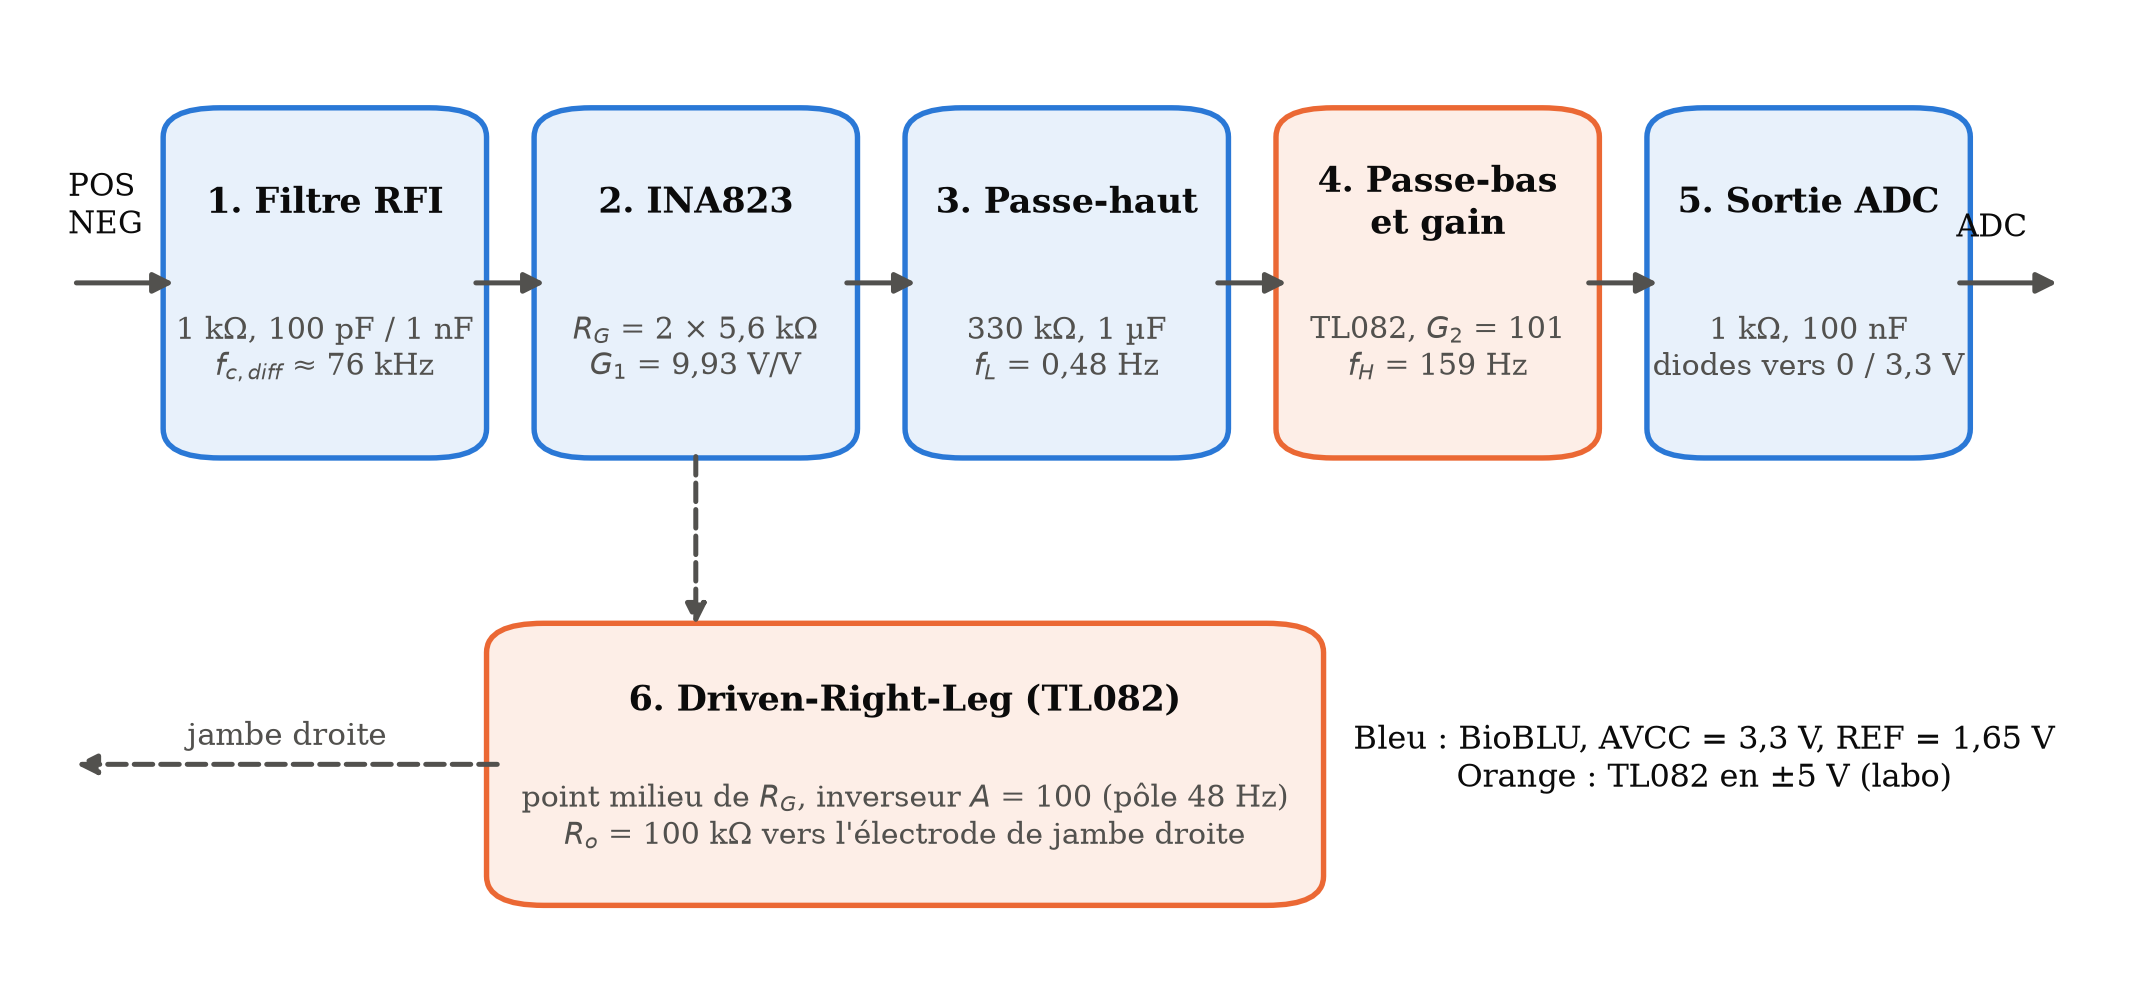
\includegraphics[width=\textwidth]{fig_6_schema_bioampli.png}
\caption{Schéma fonctionnel du bioamplificateur. Les blocs bleus sont alimentés par le BioBLU ($3,3\text{ V}$, $V_{ref} = 1,65\text{ V}$), les blocs orange (TL082) par l'alimentation $\pm 5\text{ V}$ du laboratoire, avec une masse commune.}
\label{fig:schema_bioampli}
\end{figure}

\question{6.1 (Calculs des gains et fréquences de coupure de la conception)}

\textbf{1. Filtre RFI d'entrée.}
Le filtre passif placé avant l'INA823 (notes de cours, diapositive 43, et note AN-671) empêche la rectification des signaux radiofréquence dans les jonctions d'entrée. Il comprend deux résistances séries $R = 1\text{ k}\Omega$, deux condensateurs de mode commun $C_C = 100\text{ pF}$ vers la masse et un condensateur différentiel $C_D = 1\text{ nF}$, dix fois plus grand que $C_C$ pour réduire l'effet du désappariement de $C_C$ sur le TRMC :
\begin{align*}
f_{c,\text{diff}} &= \frac{1}{2\pi \cdot 2R \cdot (C_D + C_C/2)} = \frac{1}{2\pi \times 2000\,\Omega \times 1,05\text{ nF}} \approx 75,8\text{ kHz}, \\
f_{c,\text{cm}} &= \frac{1}{2\pi R C_C} = \frac{1}{2\pi \times 1000\,\Omega \times 100\text{ pF}} \approx 1,59\text{ MHz}.
\end{align*}
La version précédente de notre conception utilisait $C_C = 1\text{ nF}$ et $C_D = 10\text{ nF}$ ($f_{c,\text{diff}} = 7,58\text{ kHz}$). Ces valeurs ont été divisées par dix parce que l'impédance des électrodes s'ajoute à $R$ : avec un déséquilibre entre les deux électrodes, les condensateurs $C_C$ forment un diviseur qui convertit le mode commun à $60\text{ Hz}$ en signal différentiel (diapositive 37), et l'effet est dix fois plus faible avec $C_C = 100\text{ pF}$ ($26,5\text{ M}\Omega$ à $60\text{ Hz}$ au lieu de $2,65\text{ M}\Omega$). La simulation (question 6.2) chiffre cet effet.

\textbf{2. Préamplificateur INA823.}
Le gain est fixé par la résistance $R_G$ entre les broches RG :
\[
G_1 = 1 + \frac{100\text{ k}\Omega}{R_G}.
\]
La valeur exacte pour $G_1 = 10$ serait $R_G = 100\text{ k}\Omega / 9 = 11,1\text{ k}\Omega$. Nous utilisons deux résistances de $5,6\text{ k}\Omega$ en série ($R_G = 11,2\text{ k}\Omega$), dont le point milieu est au potentiel de mode commun des entrées et alimente le DRL, comme au Laboratoire~1 :
\[
G_1 = 1 + \frac{100\text{ k}\Omega}{11,2\text{ k}\Omega} = 9,93\text{ V/V} \quad (19,94\text{ dB}).
\]
La broche REF est reliée à $V_{ref} = 1,65\text{ V}$.

\textbf{3. Filtre passe-haut du 1\textsuperscript{er} ordre.}
Placé après l'INA823, le condensateur série $C_H = 1\ \mu\text{F}$ et la résistance $R_H = 330\text{ k}\Omega$ vers $V_{ref}$ bloquent l'offset continu amplifié et les dérives lentes :
\[
f_L = \frac{1}{2\pi R_H C_H} = \frac{1}{2\pi \times 330\text{ k}\Omega \times 1\ \mu\text{F}} \approx 0,482\text{ Hz}, \qquad \tau = R_H C_H = 0,33\text{ s}.
\]
Le filtre est chargé par l'entrée non inverseuse du TL082 ($10^{12}\,\Omega$), ce qui ne modifie pas $f_L$.

\textbf{4. Filtre passe-bas du 1\textsuperscript{er} ordre et étage de gain (TL082).}
Un TL082 monté en non-inverseur fournit le gain et le pôle passe-bas, avec $R_1 = 1\text{ k}\Omega$ vers $V_{ref}$ et $R_f = 100\text{ k}\Omega$ en parallèle avec $C_f = 10\text{ nF}$ :
\[
G_2 = 1 + \frac{R_f}{R_1} = 101\text{ V/V} \ (40,09\text{ dB}), \qquad f_H = \frac{1}{2\pi R_f C_f} = \frac{1}{2\pi \times 100\text{ k}\Omega \times 10\text{ nF}} \approx 159,2\text{ Hz}.
\]
La fonction de transfert de ce montage est $1 + (R_f/R_1)/(1 + sR_fC_f)$ : au-delà de $f_H$, le gain diminue de $20\text{ dB/décade}$ seulement jusqu'au zéro $f_z = 1/(2\pi (R_f \parallel R_1) C_f) \approx 16,1\text{ kHz}$, puis se stabilise à $1\text{ V/V}$ ($0\text{ dB}$). L'étage seul n'atténue donc pas plus de $40\text{ dB}$. Le pôle $f_H$ dépend uniquement de $R_f C_f$; le gain est réglé par un potentiomètre de $1\text{ k}\Omega$ en série avec $R_1$ ($G_2$ de $51$ à $101\text{ V/V}$) sans déplacer $f_H$.

\textbf{5. Sortie vers l'ADC.}
Une cellule $R_{out} = 1\text{ k}\Omega$, $C_{out} = 100\text{ nF}$ prolonge l'atténuation au-delà de $f_z$ et sert de filtre anti-repliement pour l'échantillonnage du BioBLU ($2\text{ kHz}$ au Laboratoire~2) :
\[
f_{c,\text{out}} = \frac{1}{2\pi R_{out} C_{out}} \approx 1,59\text{ kHz}.
\]
Comme le TL082 est alimenté en $\pm 5\text{ V}$, deux diodes Schottky vers $0$ et $3,3\text{ V}$ limitent la tension à l'entrée de l'ADC, et $R_{out}$ limite le courant dans ces diodes.

\textbf{6. Circuit Driven-Right-Leg (DRL).}
Comme dans les notes de cours (diapositives 39 à 41), le DRL prélève la tension de mode commun sur l'étage d'entrée de l'amplificateur d'instrumentation, ici au point milieu de $R_G$, l'inverse, l'amplifie et la renvoie au corps par l'électrode de jambe droite. Le second amplificateur du TL082 est monté en inverseur avec $R_{in} = 10\text{ k}\Omega$, $R_{f,DRL} = 1\text{ M}\Omega$ et $C_{f,DRL} = 3,3\text{ nF}$ :
\begin{align*}
A_{DRL}(0) &= \frac{R_{f,DRL}}{R_{in}} = 100\text{ V/V}, \qquad f_{p,DRL} = \frac{1}{2\pi R_{f,DRL} C_{f,DRL}} \approx 48,2\text{ Hz}, \\
|A_{DRL}(60\text{ Hz})| &= \frac{100}{\sqrt{1 + (60/48,2)^2}} \approx 62,6 \ (36\text{ dB}).
\end{align*}
Le pôle $f_{p,DRL}$ fixe la bande de la boucle, qui doit rester sous les pôles formés par la résistance de protection, la capacité du corps et les électrodes pour que la boucle soit stable. Le gain de boucle extrait des simulations LTspice (question 6.2) a guidé le choix de $C_{f,DRL}$ : avec $10\text{ nF}$ ($f_{p,DRL} = 15,9\text{ Hz}$), la marge de phase était de $74^\circ$ mais le DRL n'atténuait le $60\text{ Hz}$ que de $15\text{ dB}$; avec $3,3\text{ nF}$, la marge de phase reste supérieure à $50^\circ$ pour une capacité du corps de $100$ à $300\text{ pF}$ et l'atténuation atteint $23\text{ dB}$. Avec $2,2\text{ nF}$, la marge descendrait à $44^\circ$. La résistance $R_o = 100\text{ k}\Omega$ en série avec l'électrode de jambe droite limite le courant injecté dans le corps à environ $35\ \mu\text{A}$ même si l'AOP sature (sortie à $\pm 3,4\text{ V}$); en fonctionnement normal, la sortie du DRL reste à quelques millivolts de $V_{ref}$. Les notes de cours suggèrent une valeur plus grande ($\approx 5\text{ M}\Omega$) pour un appareil certifié, au prix d'une réjection plus faible. La résistance effective entre le corps et $V_{ref}$ devient (diapositive 41)
\[
R_{\text{eff}} = \frac{|Z_{RL}| + R_o}{1 + |A_{DRL}|} \approx \frac{38\text{ k}\Omega + 100\text{ k}\Omega}{63,6} \approx 2,2\text{ k}\Omega \text{ à } 60\text{ Hz},
\]
contre $|Z_{RL}| \approx 38\text{ k}\Omega$ (électrode de $51\text{ k}\Omega \parallel 47\text{ nF}$) lorsque la jambe droite est reliée directement à $V_{ref}$, soit une réduction attendue de la tension de mode commun d'environ $25\text{ dB}$ (le calcul néglige les phases; la simulation donne $23\text{ dB}$).

\textbf{7. Synthèse.}
\begin{align*}
A_{v,\text{total}} &= G_1 \times G_2 = 9,93 \times 101 \approx 1003\text{ V/V} \ (60,0\text{ dB}), \\
f_L &= 0,48\text{ Hz}, \qquad f_H \approx 159\text{ Hz} \ (\text{légèrement abaissée par la cellule de sortie}).
\end{align*}

\begin{table}[H]
\centering
\caption{Dimensionnement des composants et valeurs calculées pour chaque étage.}
\label{tab:dimensionnement}
\small
\begin{tabular}{p{2.6cm}p{5.6cm}p{2.4cm}p{3.6cm}}
\toprule
\textbf{Étage} & \textbf{Composants} & \textbf{Gain} & \textbf{Fréquence(s)} \\
\midrule
1. Filtre RFI & $R = 1\text{ k}\Omega$, $C_C = 100\text{ pF}$, $C_D = 1\text{ nF}$ & $0\text{ dB}$ & $f_{c,\text{diff}} = 75,8\text{ kHz}$, $f_{c,\text{cm}} = 1,59\text{ MHz}$ \\
2. INA823 & $R_G = 2 \times 5,6\text{ k}\Omega$, REF à $1,65\text{ V}$ & $19,94\text{ dB}$ ($9,93\text{ V/V}$) & -- \\
3. Passe-haut & $C_H = 1\ \mu\text{F}$, $R_H = 330\text{ k}\Omega$ & $0\text{ dB}$ & $f_L = 0,482\text{ Hz}$ \\
4. Passe-bas et gain & $R_1 = 1\text{ k}\Omega$ (+ pot. $1\text{ k}\Omega$), $R_f = 100\text{ k}\Omega$, $C_f = 10\text{ nF}$ & $40,09\text{ dB}$ ($101\text{ V/V}$) & $f_H = 159,2\text{ Hz}$, $f_z = 16,1\text{ kHz}$ \\
5. Sortie ADC & $R_{out} = 1\text{ k}\Omega$, $C_{out} = 100\text{ nF}$, 2 diodes Schottky & $0\text{ dB}$ & $f_{c,\text{out}} = 1,59\text{ kHz}$ \\
6. DRL & $R_{in} = 10\text{ k}\Omega$, $R_{f,DRL} = 1\text{ M}\Omega$, $C_{f,DRL} = 3,3\text{ nF}$, $R_o = 100\text{ k}\Omega$ & $40\text{ dB}$ en DC, $36\text{ dB}$ à $60\text{ Hz}$ & $f_{p,DRL} = 48,2\text{ Hz}$ \\
\midrule
\textbf{Chaîne} & & \textbf{60,0 dB} & \textbf{0,48 à $\approx$159 Hz} \\
\bottomrule
\end{tabular}
\end{table}

\question{6.2 (Diagrammes de Bode dans LTspice selon l'approche systémique)}

Les simulations utilisent les modèles TI de l'INA823 et du TL082 dans LTspice~26 (dossier \texttt{ltspice/}). Conformément à l'approche systémique, chaque diagramme de Bode est le rapport entre la tension de sortie et la tension d'entrée de l'étage : $V(OUT)/(V(POS)-V(NEG))$ en mode différentiel et $V(OUT)/\tfrac{V(POS)+V(NEG)}{2}$ en mode commun. Ces expressions s'affichent directement dans LTspice (\og Add Trace \fg{}); les figures ci-dessous les retracent à partir des fichiers \texttt{.raw} de LTspice. Sauf mention contraire, l'INA823 est alimenté par le BioBLU ($3,3\text{ V}$, $V_{ref} = 1,65\text{ V}$) et les TL082 en $\pm 5\text{ V}$.

\textbf{1. Préamplificateur INA823.}
Le balayage DC de la Figure~\ref{fig:offset} applique un offset continu entre les deux entrées. La sortie suit $V_{ref} + G_1 V_{off}$ avec un gain petit signal de $9,93\text{ V/V}$ tant que l'offset reste entre $-164$ et $+161\text{ mV}$, puis se fixe à $0,02\text{ V}$ ou $3,25\text{ V}$ (sortie rail à rail) et le gain devient nul : l'ECG disparaît. Cette plage est celle utilisée à la section 5.

\begin{figure}[!htb]
\centering
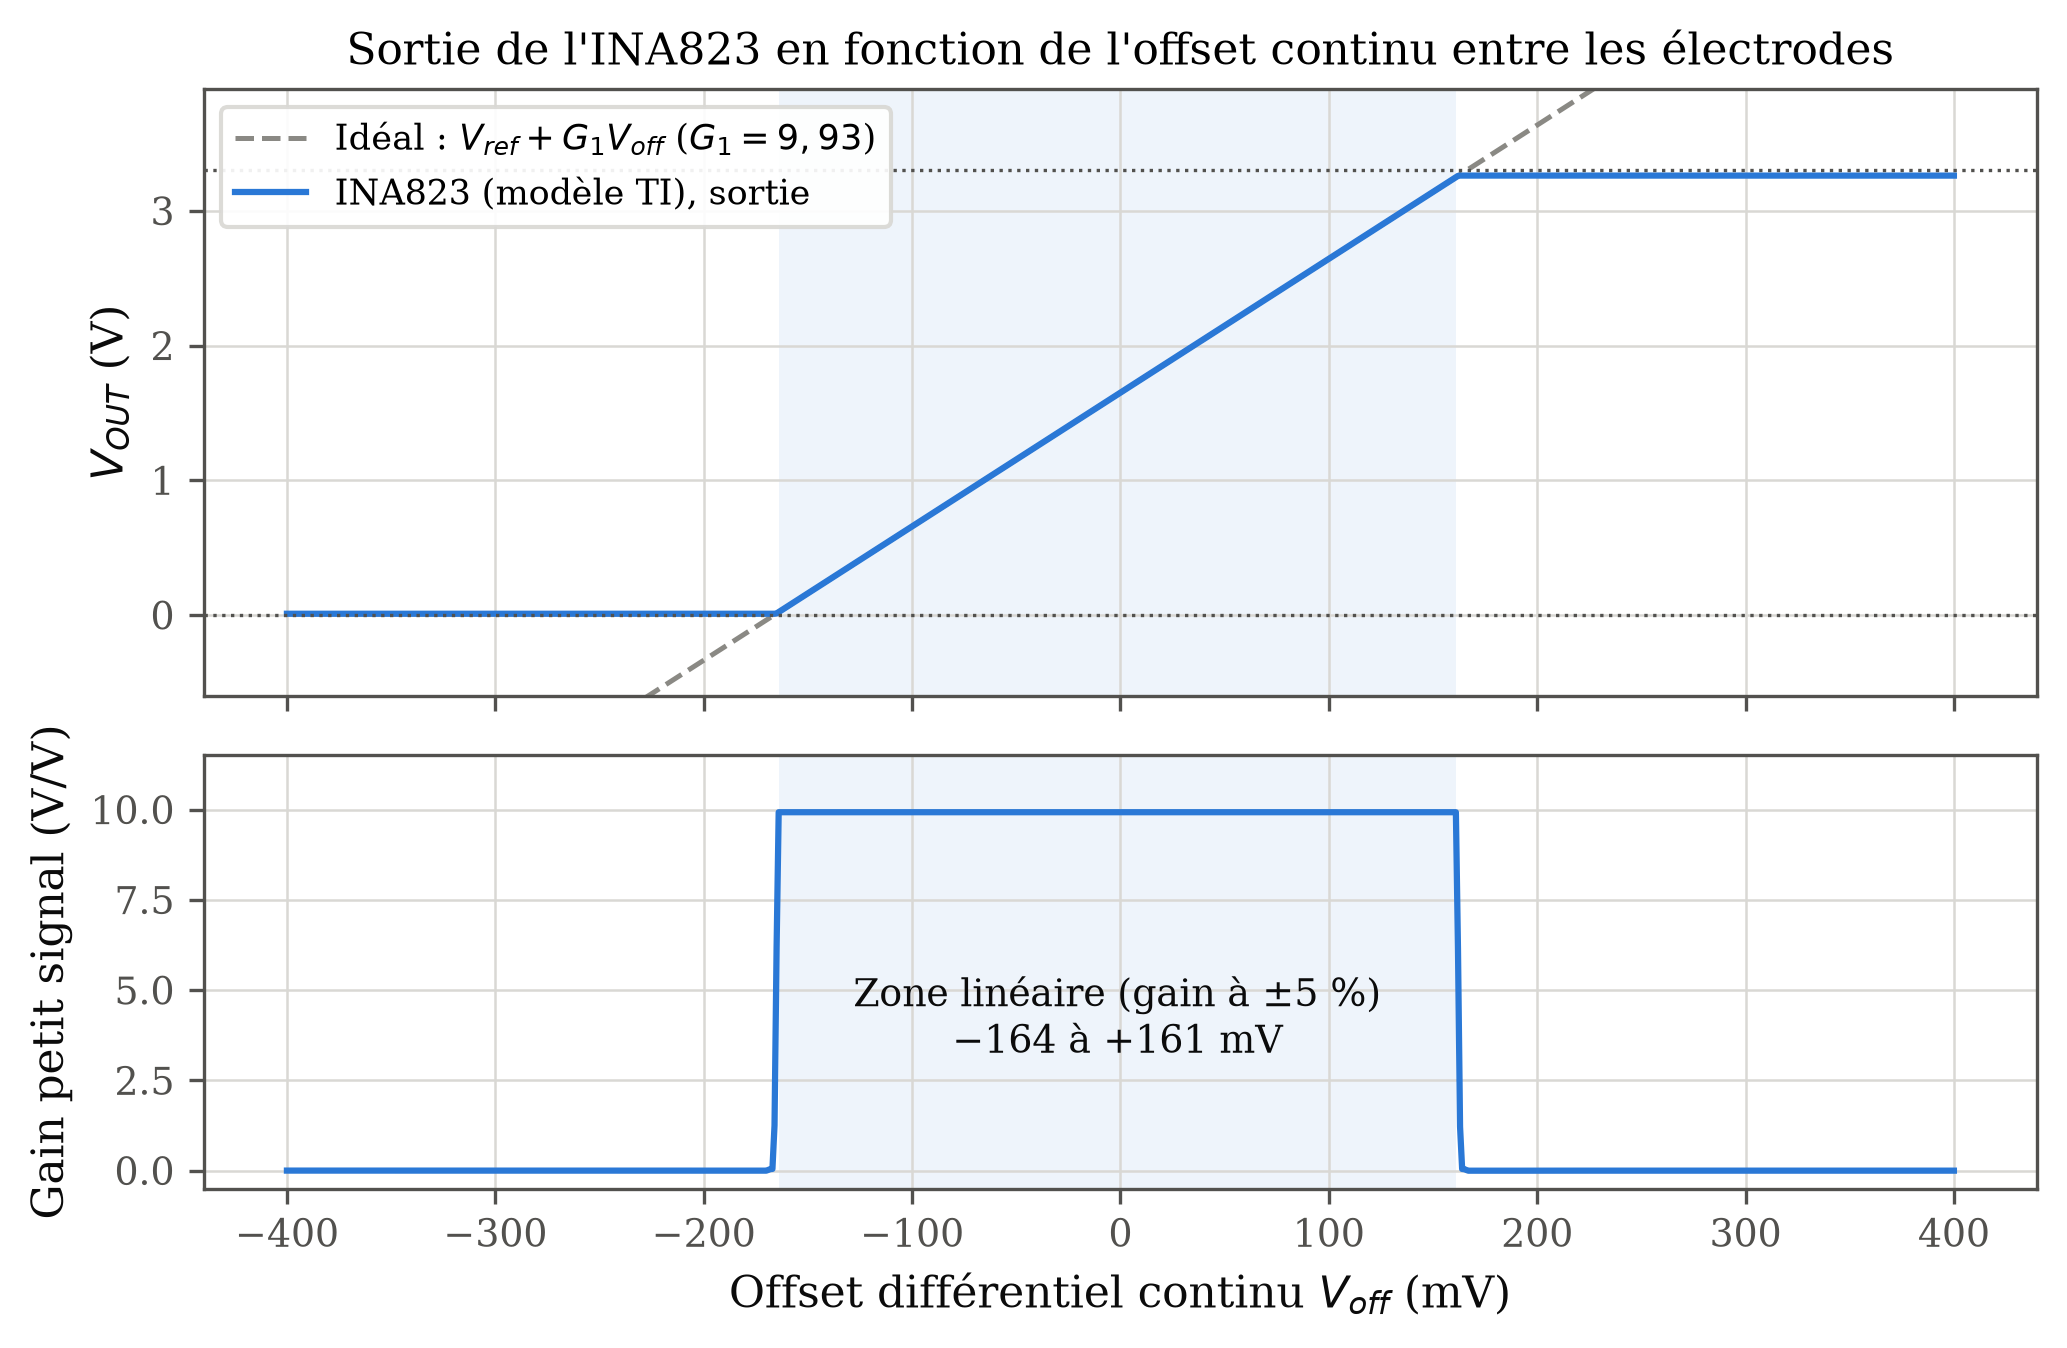
\includegraphics[width=0.88\textwidth]{fig_6_1_offset_ina823.png}
\caption{Sortie de l'INA823 ($G_1 = 9,93$, alimentation $3,3\text{ V}$) en fonction de l'offset continu entre les électrodes (balayage DC, modèle TI). Bas : gain petit signal $dV_{OUT}/dV_{off}$; zone linéaire en bleu.}
\label{fig:offset}
\end{figure}

La Figure~\ref{fig:bode_ina} présente les gains différentiel et de mode commun. Le gain différentiel vaut $19,94\text{ dB}$ ($9,93\text{ V/V}$) et reste plat jusqu'à environ $500\text{ kHz}$ ($-3\text{ dB}$ à $517\text{ kHz}$). Le gain de mode commun vaut $-110\text{ dB}$ à basse fréquence et $-105,4\text{ dB}$ à $60\text{ Hz}$. Le TRMC du modèle est donc de $130\text{ dB}$ à $1\text{ Hz}$, $125,4\text{ dB}$ à $60\text{ Hz}$ et $103\text{ dB}$ à $1\text{ kHz}$. Ce sont des valeurs typiques du modèle : en pratique, le rejet du mode commun sera surtout limité par le déséquilibre des électrodes (point 4).

\begin{figure}[H]
\centering
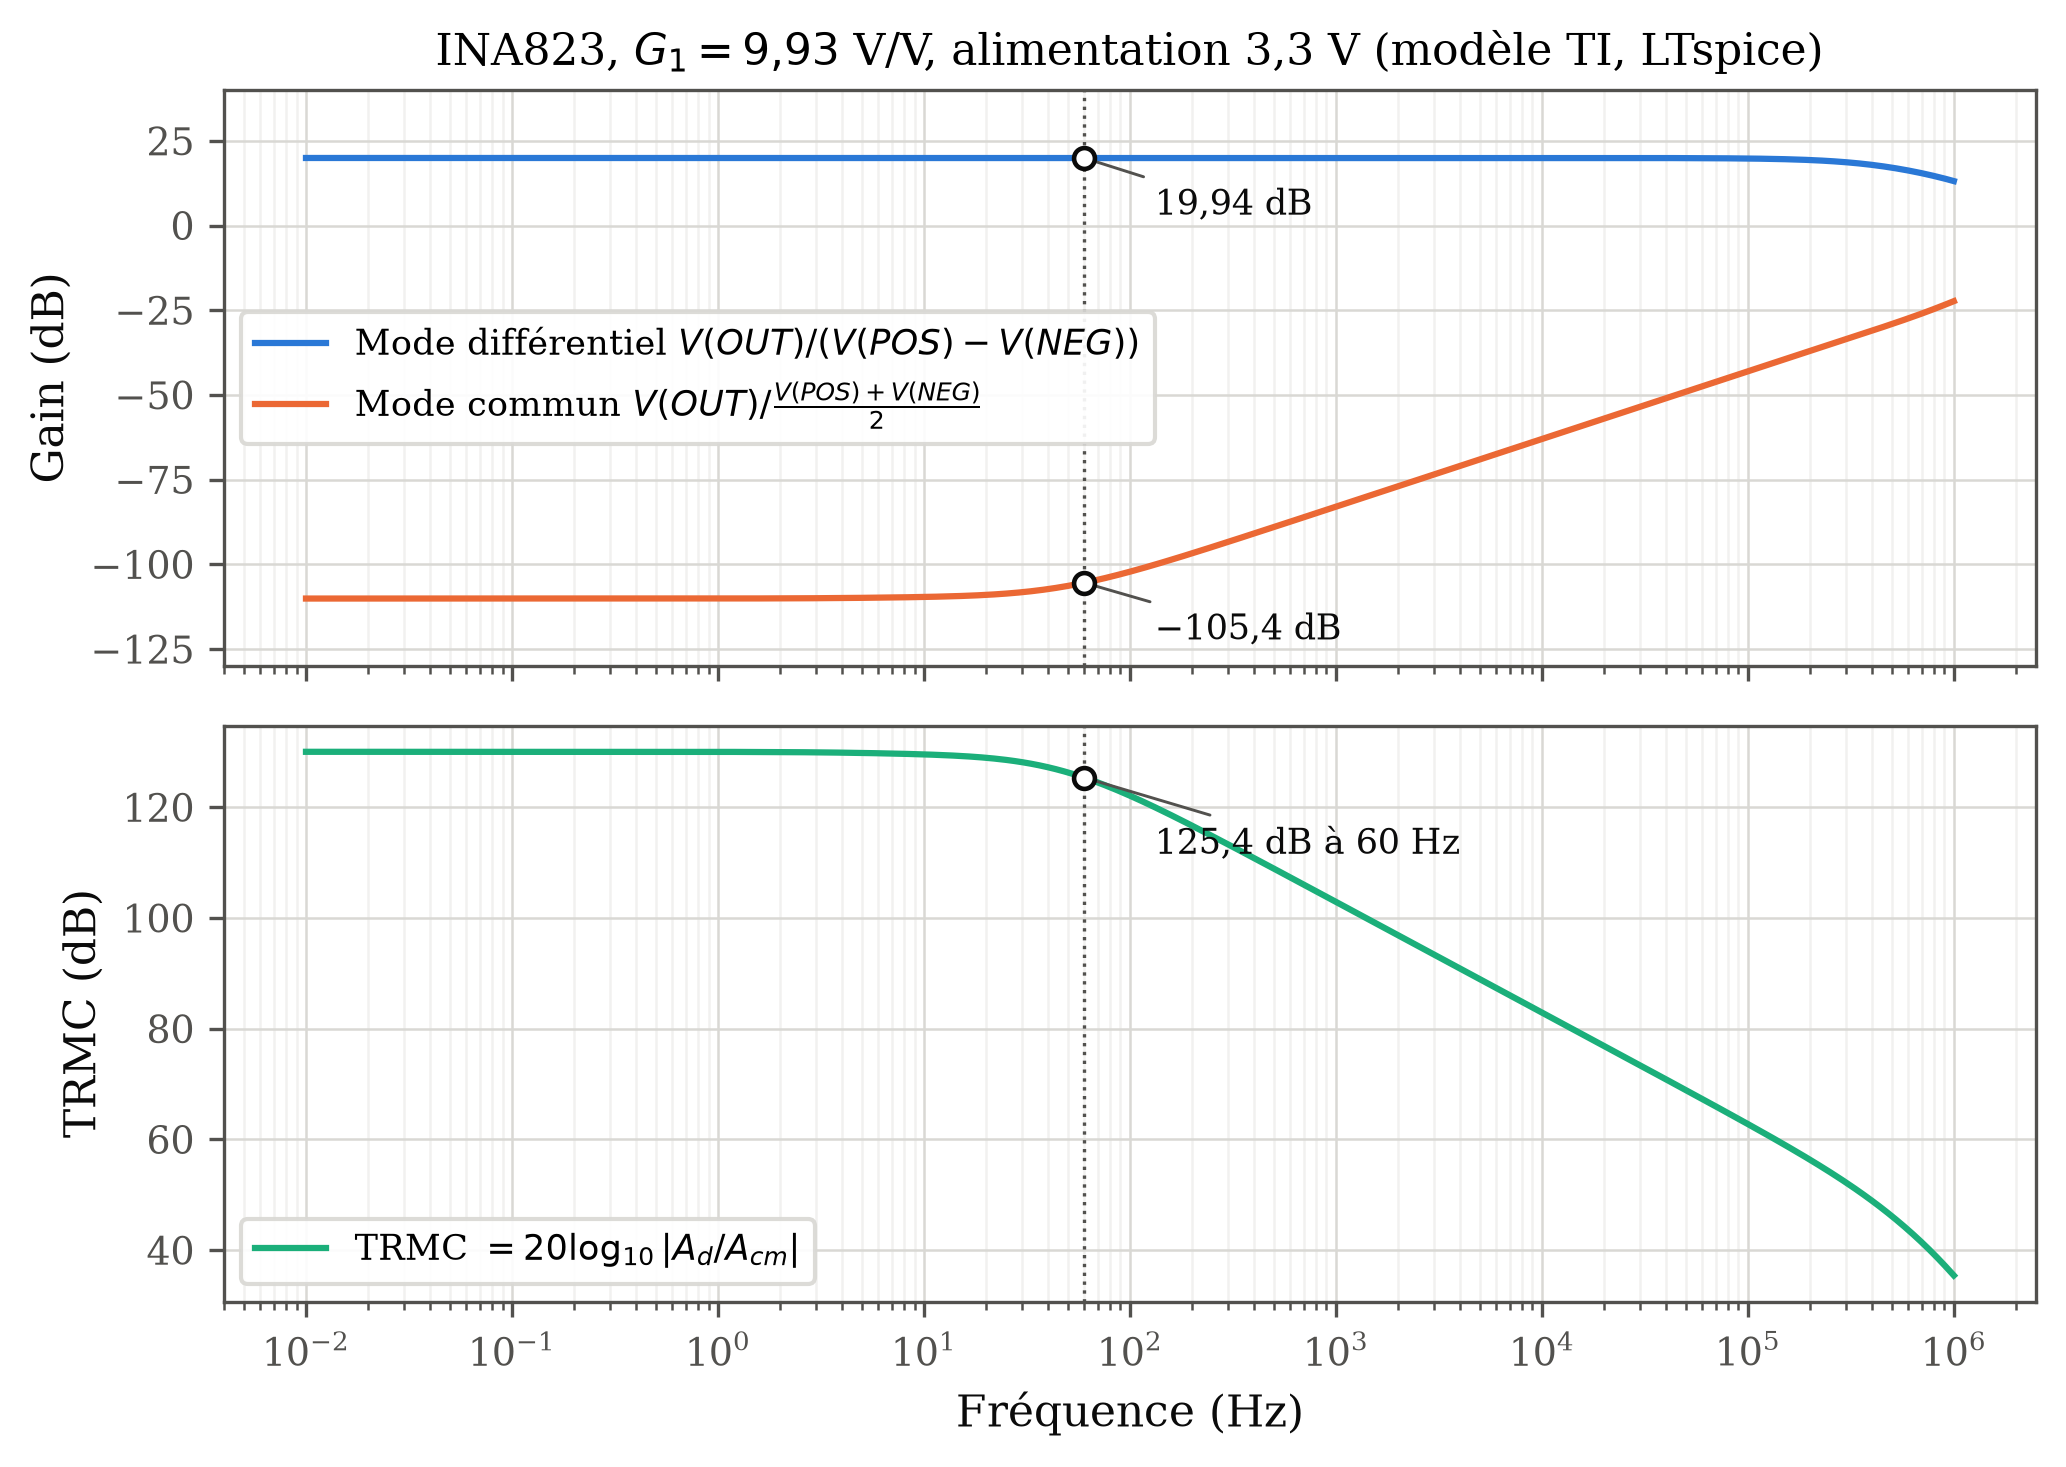
\includegraphics[width=0.88\textwidth]{fig_6_2a_bode_ina823.png}
\caption{Diagramme de Bode de l'INA823 selon l'approche systémique (LTspice, modèle TI). Haut : gain différentiel et gain de mode commun. Bas : TRMC $= 20\log_{10}|A_d/A_{cm}|$.}
\label{fig:bode_ina}
\end{figure}

\textbf{2. Filtres pris isolément.}
La Figure~\ref{fig:bode_filtres} donne la réponse de chaque filtre.
\begin{itemize}
\item \textit{Filtre RFI} (a) : avec une source idéale, $f_{c,\text{diff}} = 75,6\text{ kHz}$, conforme au calcul ($75,8\text{ kHz}$). À travers deux électrodes ($51\text{ k}\Omega \parallel 47\text{ nF}$), la coupure descend à $60\text{ kHz}$ et la perte à $150\text{ Hz}$ n'est que de $0,32\text{ dB}$. Avec les valeurs de la version précédente ($C_C = 1\text{ nF}$, $C_D = 10\text{ nF}$), l'impédance des électrodes ramène la coupure à $201\text{ Hz}$, avec $-2,8\text{ dB}$ à $150\text{ Hz}$ : ce filtre aurait coupé dans la bande de l'ECG, ce qui justifie les nouvelles valeurs.
\item \textit{Passe-haut} (b) : $f_L = 0,484\text{ Hz}$, pente de $+20\text{ dB/décade}$, gain unitaire dans la bande.
\item \textit{Passe-bas et gain} (b) : avec le TL082 en $\pm 5\text{ V}$, le gain est de $40,08\text{ dB}$ et $f_H = 158\text{ Hz}$. Comme prévu, le gain ne descend pas sous $0\text{ dB}$ (soit $-40\text{ dB}$ normalisé) au-delà d'environ $16\text{ kHz}$.
\item \textit{RC de sortie} (b) : $f_{c,\text{out}} = 1,59\text{ kHz}$; il continue l'atténuation là où l'étage de gain plafonne.
\item \textit{TL082 sur $3,3\text{ V}$} (b, tireté) : le même étage alimenté par le BioBLU n'a plus que $9\text{ dB}$ de gain ($31\text{ dB}$ sous la valeur prévue). La sortie du modèle est bloquée près de $1,65\text{ V}$ et le gain vu en petit signal n'a plus de sens. C'est la raison de l'alimentation $\pm 5\text{ V}$ retenue à la section 5.
\end{itemize}

\begin{figure}[H]
\centering
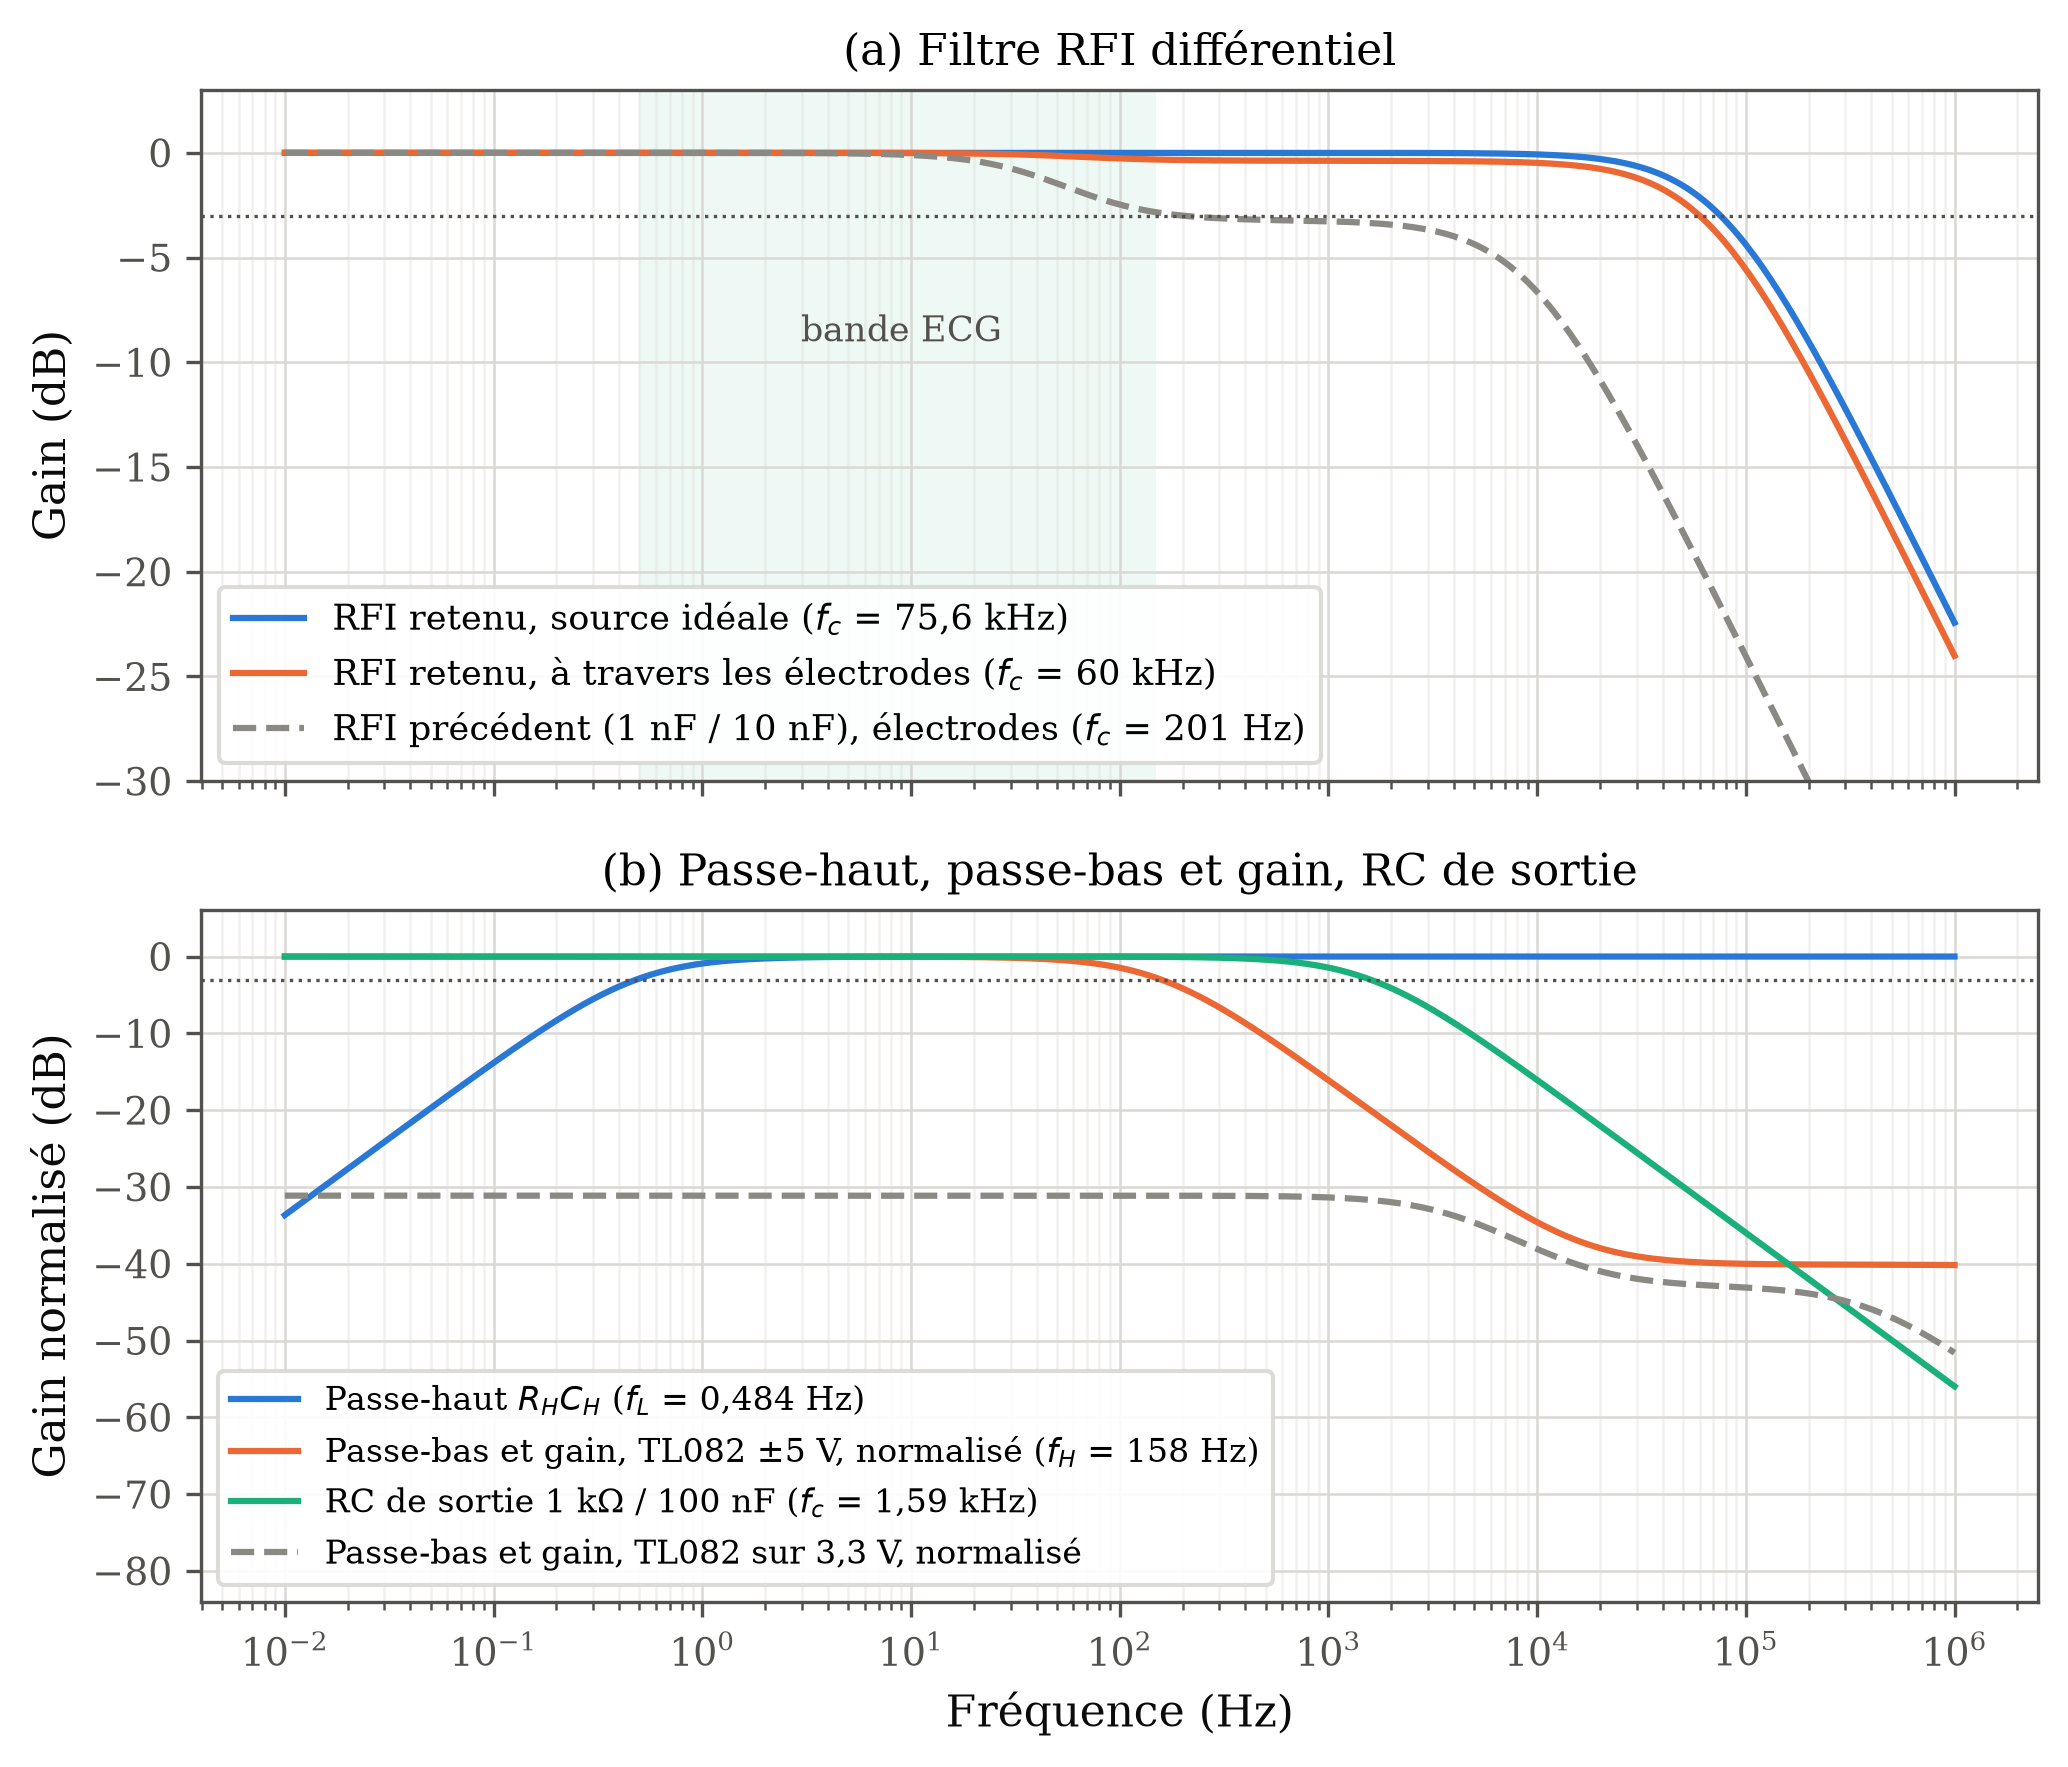
\includegraphics[width=0.88\textwidth]{fig_6_2b_bode_filtres.png}
\caption{Diagrammes de Bode des filtres pris isolément (LTspice). (a) Filtre RFI différentiel : valeurs retenues avec une source idéale et à travers les électrodes, et valeurs précédentes à travers les électrodes. (b) Passe-haut, passe-bas et gain (normalisé par $G_2 = 101$) avec le TL082 en $\pm 5\text{ V}$ et sur $3,3\text{ V}$, et RC de sortie.}
\label{fig:bode_filtres}
\end{figure}

\textbf{3. Bioamplificateur complet.}
La Figure~\ref{fig:bode_global} donne la réponse de la chaîne complète (patient, électrodes, filtre RFI, INA823, filtres, gain, sortie et DRL). Le gain maximal est de $59,99\text{ dB}$ ($999\text{ V/V}$), les coupures à $-3\text{ dB}$ sont à $f_L = 0,481\text{ Hz}$ et $f_H = 157,5\text{ Hz}$, soit une bande passante de $157\text{ Hz}$, conforme au Tableau~\ref{tab:specifications} ($60\text{ dB}$, $0,5$ à $150\text{ Hz}$). Vu de la peau, à travers l'impédance des électrodes, $f_H$ descend à $146\text{ Hz}$. Au-delà de $f_H$, le gain tombe à $42,5\text{ dB}$ à $1\text{ kHz}$ et $9,3\text{ dB}$ à $10\text{ kHz}$. La phase vaut $+45^\circ$ à $f_L$, $-50^\circ$ à $f_H$ et seulement $-6,5^\circ$ à $20\text{ Hz}$, ce qui préserve la forme du complexe QRS. Lorsque tout le circuit est alimenté en $3,3\text{ V}$, le gain dans la bande n'est que de $28,9\text{ dB}$.

\begin{figure}[H]
\centering
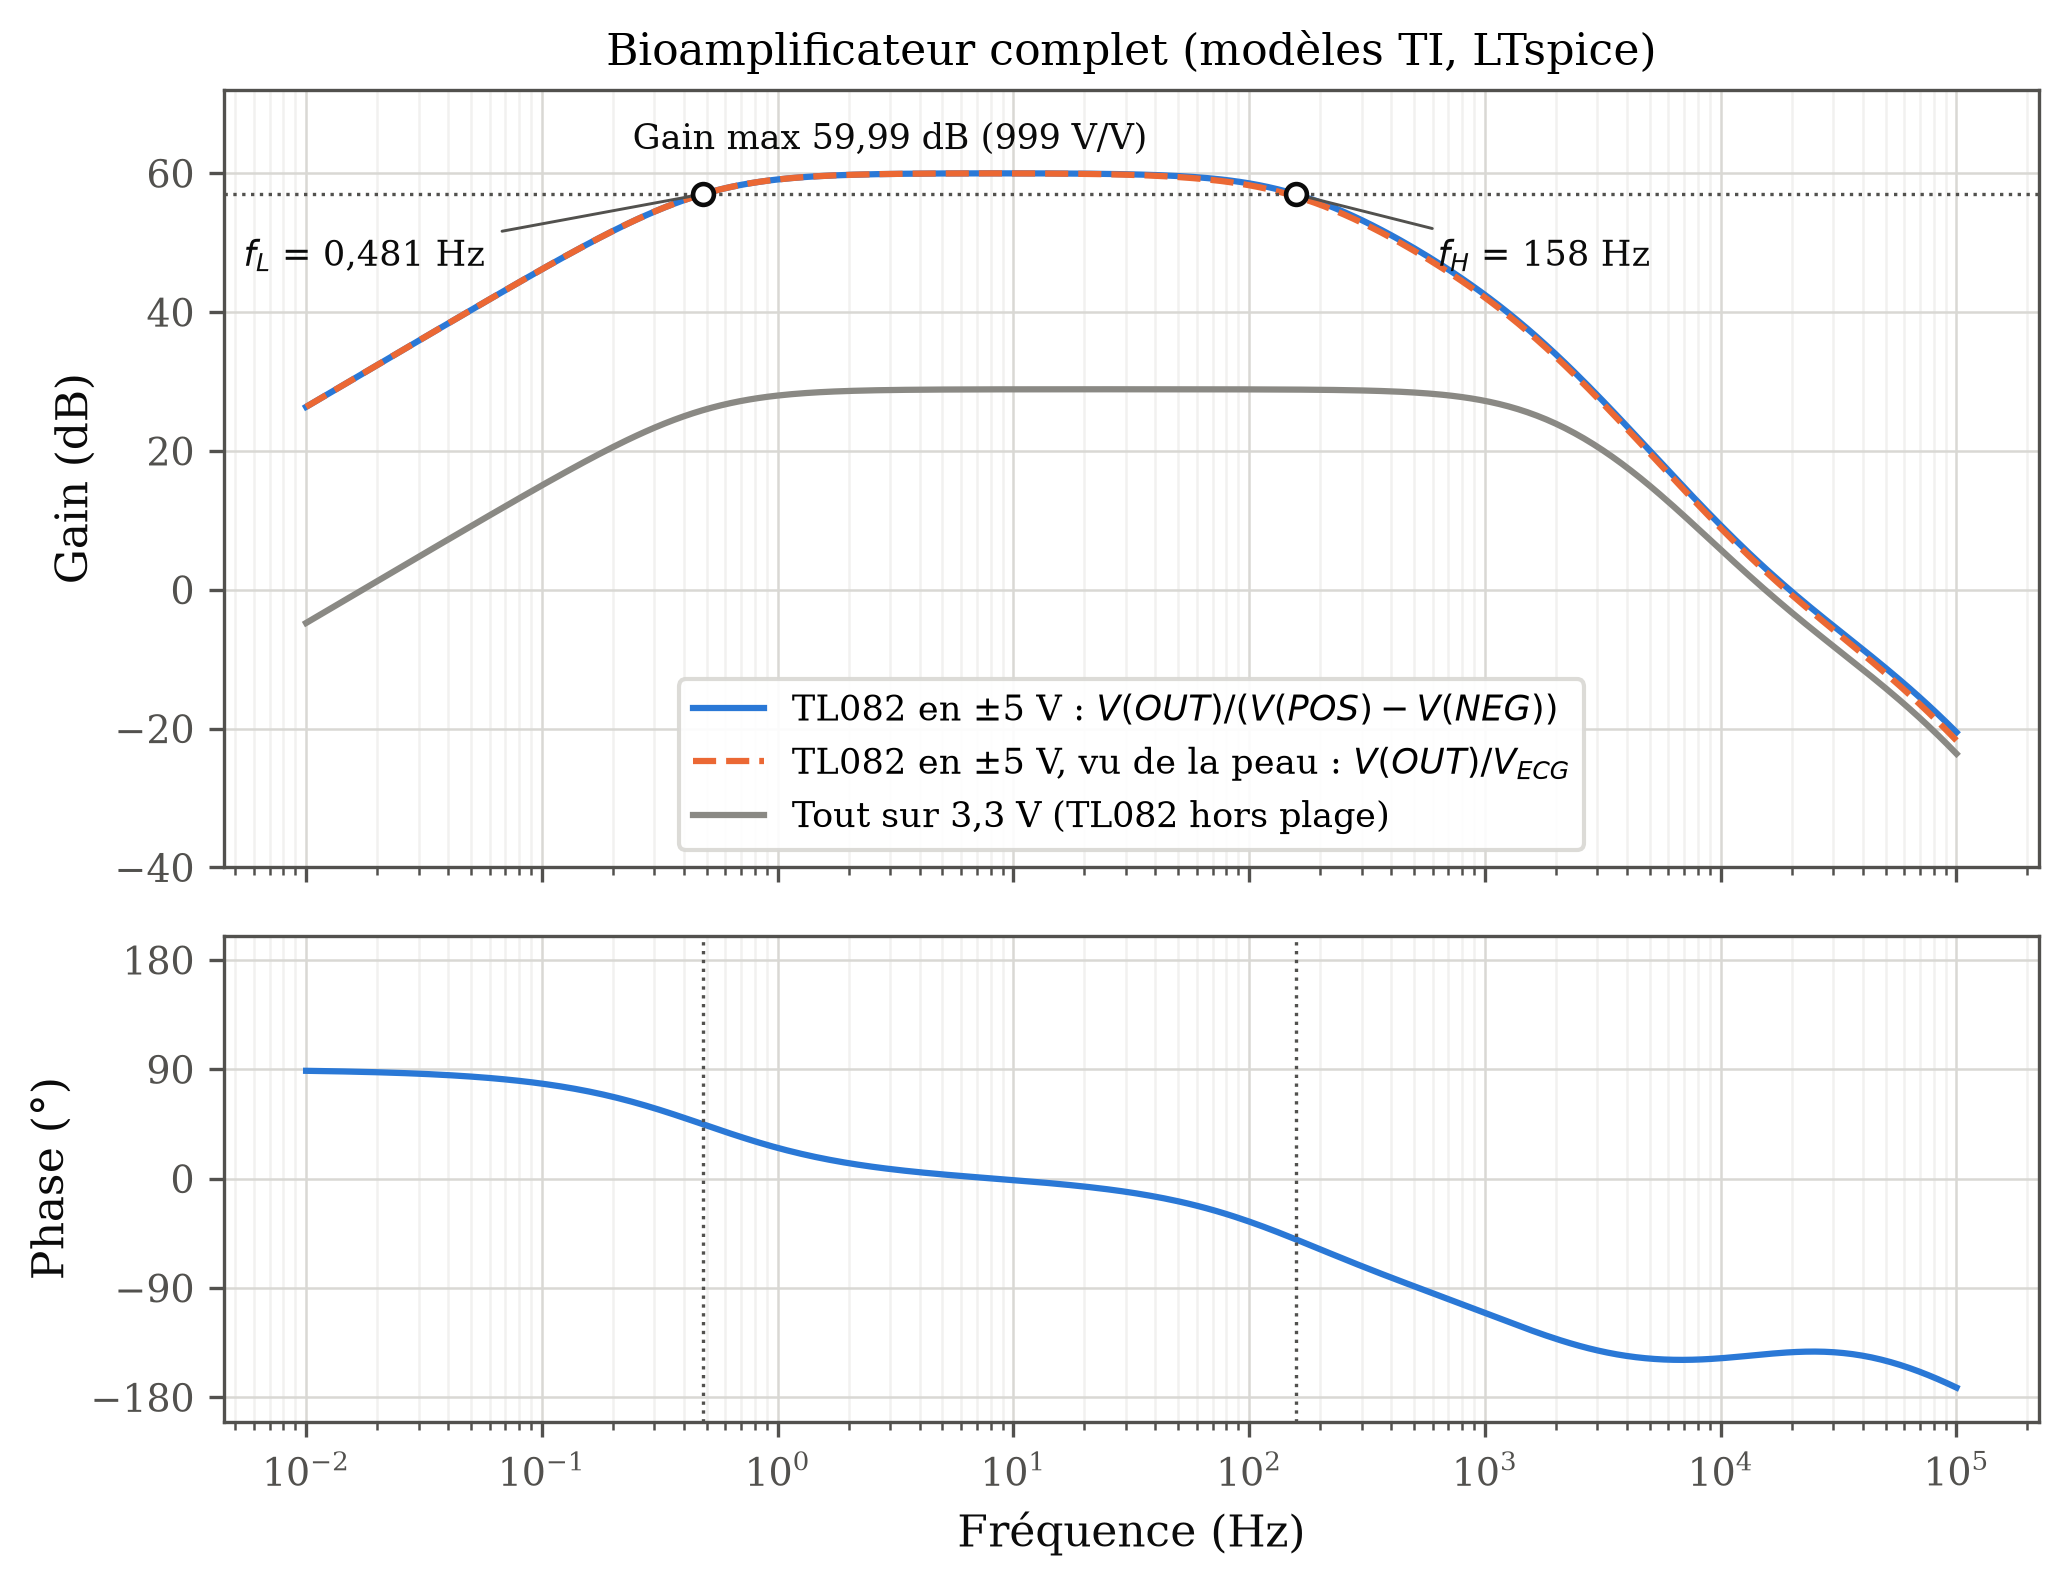
\includegraphics[width=0.9\textwidth]{fig_6_2c_bode_global.png}
\caption{Diagramme de Bode du bioamplificateur complet (LTspice, modèles TI). Haut : gain du circuit $V(OUT)/(V(POS)-V(NEG))$ et gain vu de la peau $V(OUT)/V_{ECG}$ avec les TL082 en $\pm 5\text{ V}$, et gain lorsque tout le circuit est sur $3,3\text{ V}$. Bas : phase du montage en $\pm 5\text{ V}$.}
\label{fig:bode_global}
\end{figure}

\textbf{4. Circuit Driven-Right-Leg.}
Le courant de déplacement du secteur est modélisé par une source de $0,2\ \mu\text{A}$ injectée dans le corps (notes de cours, diapositives 36 et 41), avec une capacité corps-terre de $200\text{ pF}$ et une électrode NEG $20\,\%$ plus faible que POS pour convertir le mode commun en signal différentiel. La Figure~\ref{fig:bode_drl} compare le DRL actif à une électrode de jambe droite reliée directement à $V_{ref}$. À $60\text{ Hz}$, la tension de mode commun du corps passe de $7,57$ à $0,53\text{ mV}$ ($-23,1\text{ dB}$) et le $60\text{ Hz}$ parasite en sortie de $1,74$ à $0,12\text{ mV}$. Avec le filtre RFI précédent ($C_C = 1\text{ nF}$), ce parasite serait de $0,96\text{ mV}$ même avec le DRL : le déséquilibre des électrodes et les condensateurs $C_C$ convertissent huit fois plus de mode commun en signal différentiel, ce qui confirme le choix de $C_C = 100\text{ pF}$.

La stabilité du DRL a été vérifiée à partir des mêmes données. Si l'AOP du DRL était inactif, le corps ne verrait que des éléments passifs (impédance $Z_p$ : $R_o$ et électrode de jambe droite, capacité du corps, entrées); avec le DRL, l'impédance devient $Z_{DRL} = Z_p/(1+L)$, d'où le gain de boucle $L = Z_p/Z_{DRL} - 1$. On obtient $|L| = 33,7\text{ dB}$ à $60\text{ Hz}$, un gain de boucle unitaire vers $3,0\text{ kHz}$ et une marge de phase de $54^\circ$. Au-dessus d'environ $1\text{ kHz}$, le gain du DRL s'annule et le corps n'est plus relié à $V_{ref}$ que par $R_o = 100\text{ k}\Omega$ : la tension de mode commun dépasse alors celle obtenue sans DRL (maximum de $19,7\text{ mV}$ vers $3,8\text{ kHz}$). Ce n'est pas une résonance mais la réponse passive à travers $R_o$; elle est hors de la bande de l'ECG et le parasite résultant en sortie reste inférieur à $0,05\text{ mV}$.

\begin{figure}[H]
\centering
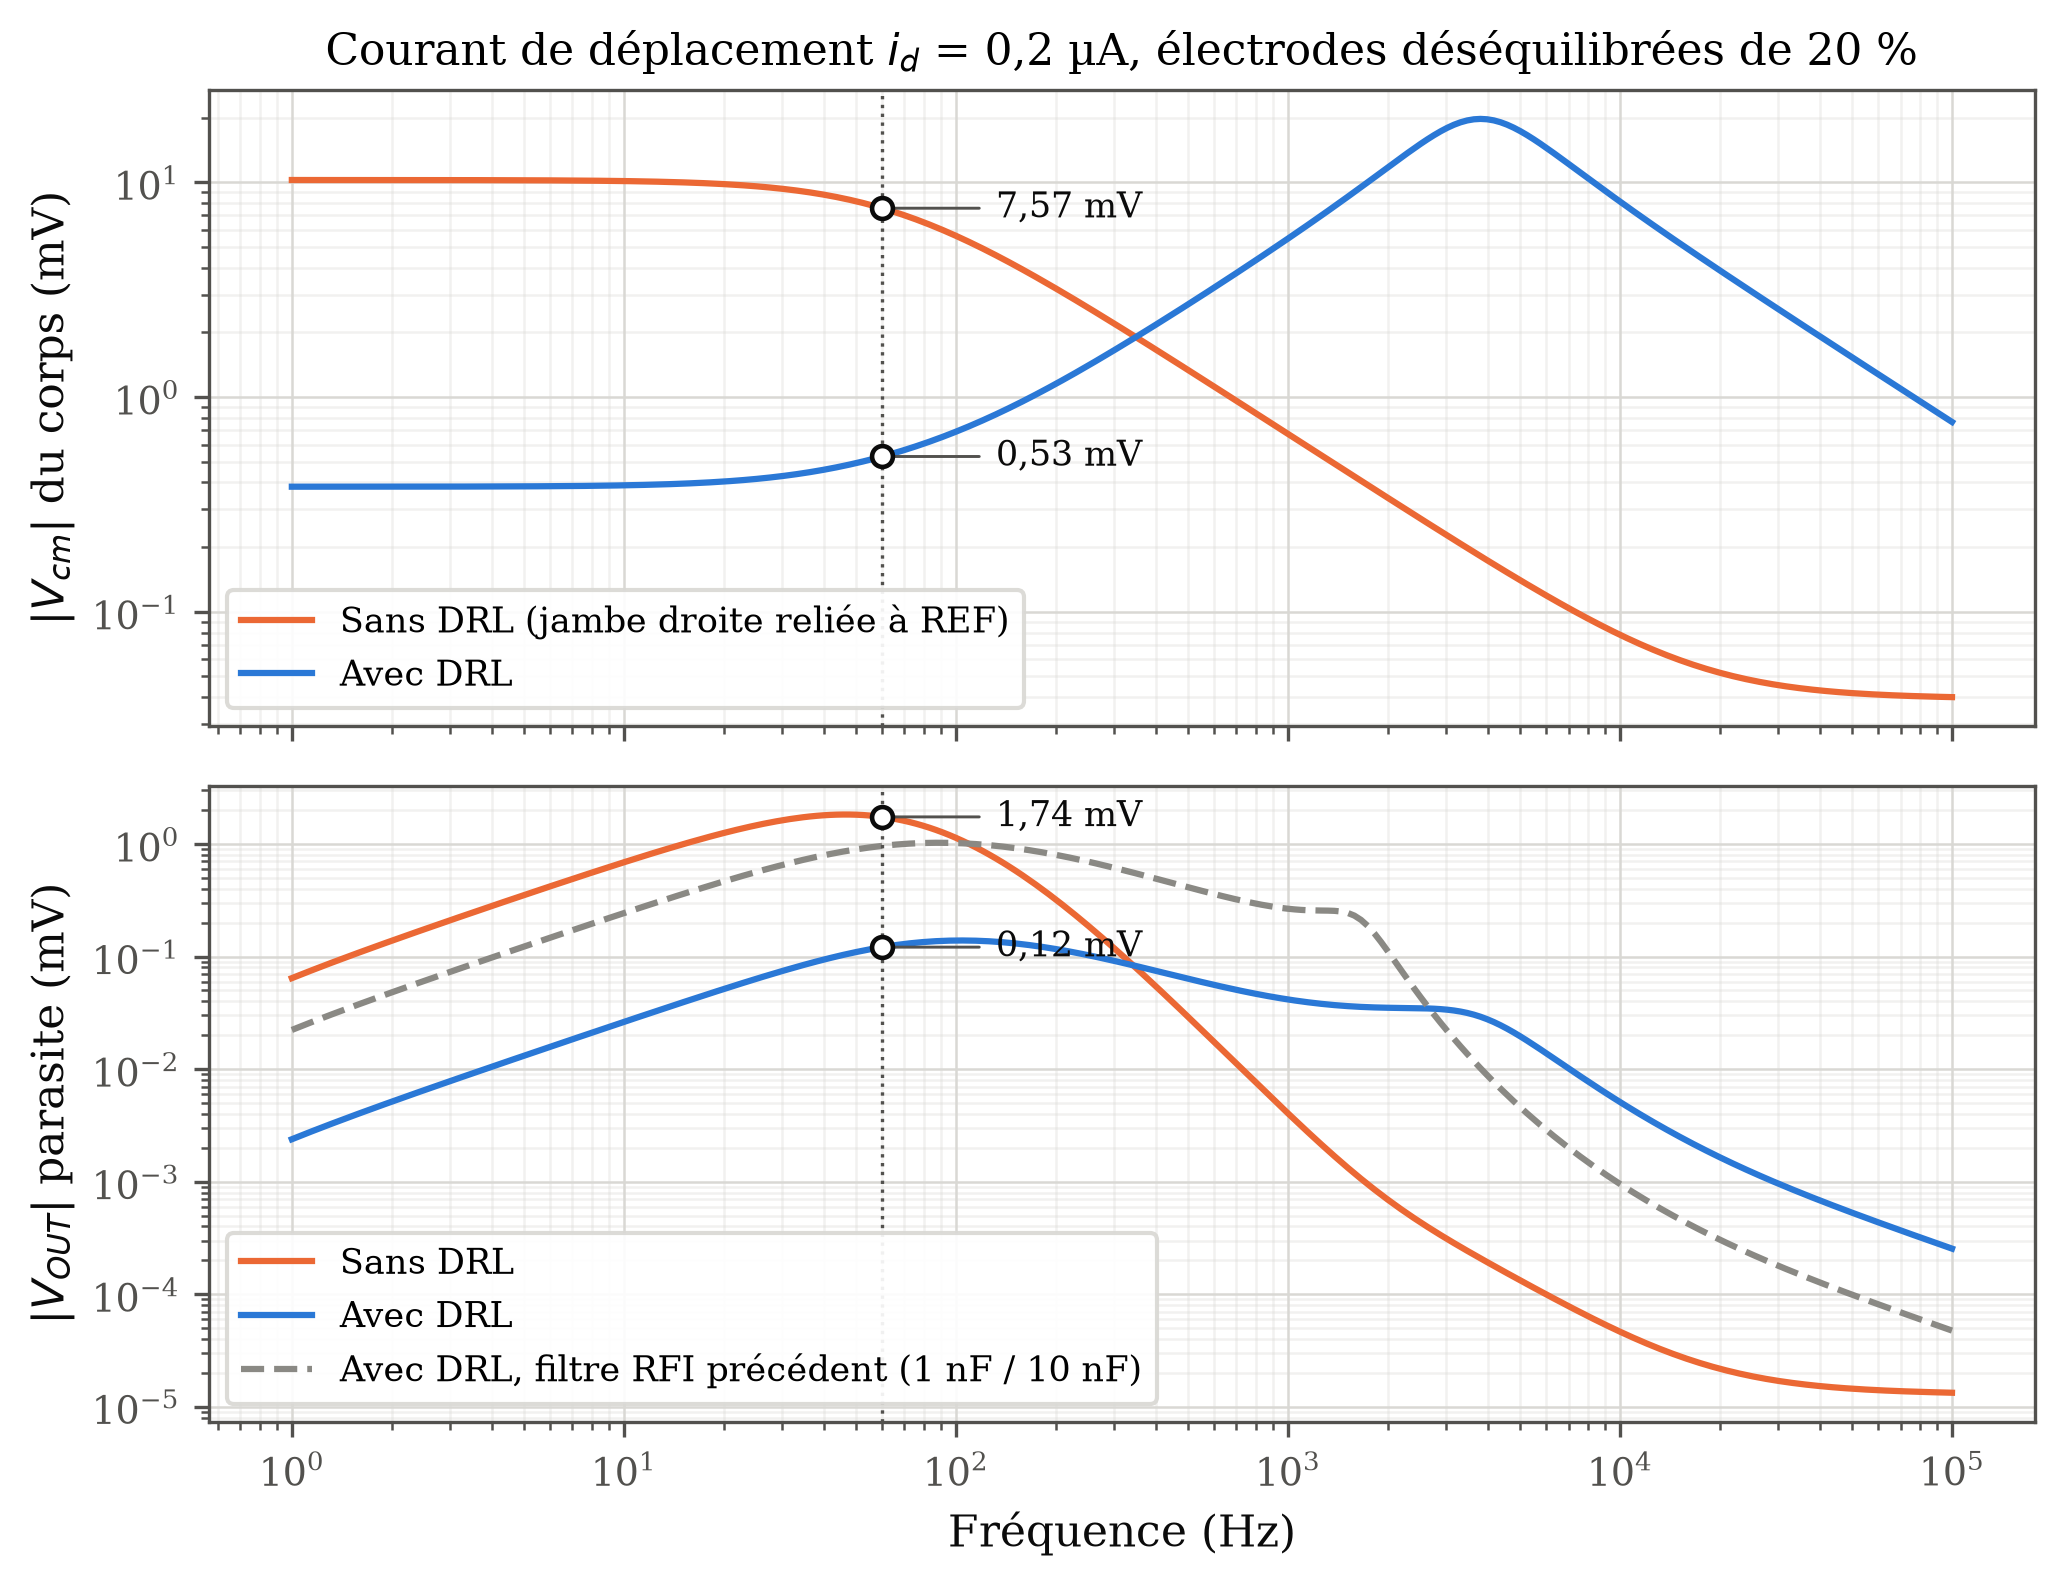
\includegraphics[width=0.88\textwidth]{fig_6_2d_drl.png}
\caption{Effet du Driven-Right-Leg (LTspice, TL082 en $\pm 5\text{ V}$). Haut : tension de mode commun du corps pour $i_d = 0,2\ \mu\text{A}$. Bas : tension parasite à la sortie du bioamplificateur, avec le filtre RFI retenu et avec le filtre RFI précédent.}
\label{fig:bode_drl}
\end{figure}

\textbf{5. Simulation temporelle.}
La Figure~\ref{fig:sim_temporelle} applique un ECG synthétique (onde R de $1,2\text{ mV}$, $68\text{ battements/min}$) superposé à un offset continu de $50\text{ mV}$ entre les électrodes, à une dérive respiratoire de $0,5\text{ mV}$ à $0,25\text{ Hz}$ et au courant de déplacement de $0,2\ \mu\text{A}$ à $60\text{ Hz}$, avec les électrodes déséquilibrées. Le point de fonctionnement initial charge $C_H$, de sorte que la simulation part du régime établi.
\begin{itemize}
\item La sortie de l'INA823 se place à $2,15\text{ V}$ ($1,65\text{ V} + 9,93 \times 50\text{ mV}$) et varie entre $2,138$ et $2,163\text{ V}$ : l'offset est amplifié sans saturation.
\item Avec les TL082 en $\pm 5\text{ V}$, la sortie vers l'ADC varie entre $1,05$ et $2,91\text{ V}$ : les ondes P, QRS et T sont nettes, le $60\text{ Hz}$ n'est pas visible et le signal reste dans la plage $0$ à $3,3\text{ V}$ de l'ADC. La dérive respiratoire, à $0,25\text{ Hz}$ sous $f_L$, est atténuée d'environ $7\text{ dB}$ et reste visible comme une lente ondulation de la ligne de base. Le pic de l'onde R, à $0,4\text{ V}$ du rail, montre qu'une onde R plus grande (dérivation II) demandera de réduire $G_2$ avec le potentiomètre.
\item Lorsque tout le circuit est alimenté en $3,3\text{ V}$, la sortie reste entre $1,63$ et $1,68\text{ V}$ : le TL082 ne peut pas fonctionner sur l'alimentation du BioBLU.
\end{itemize}

\begin{figure}[H]
\centering
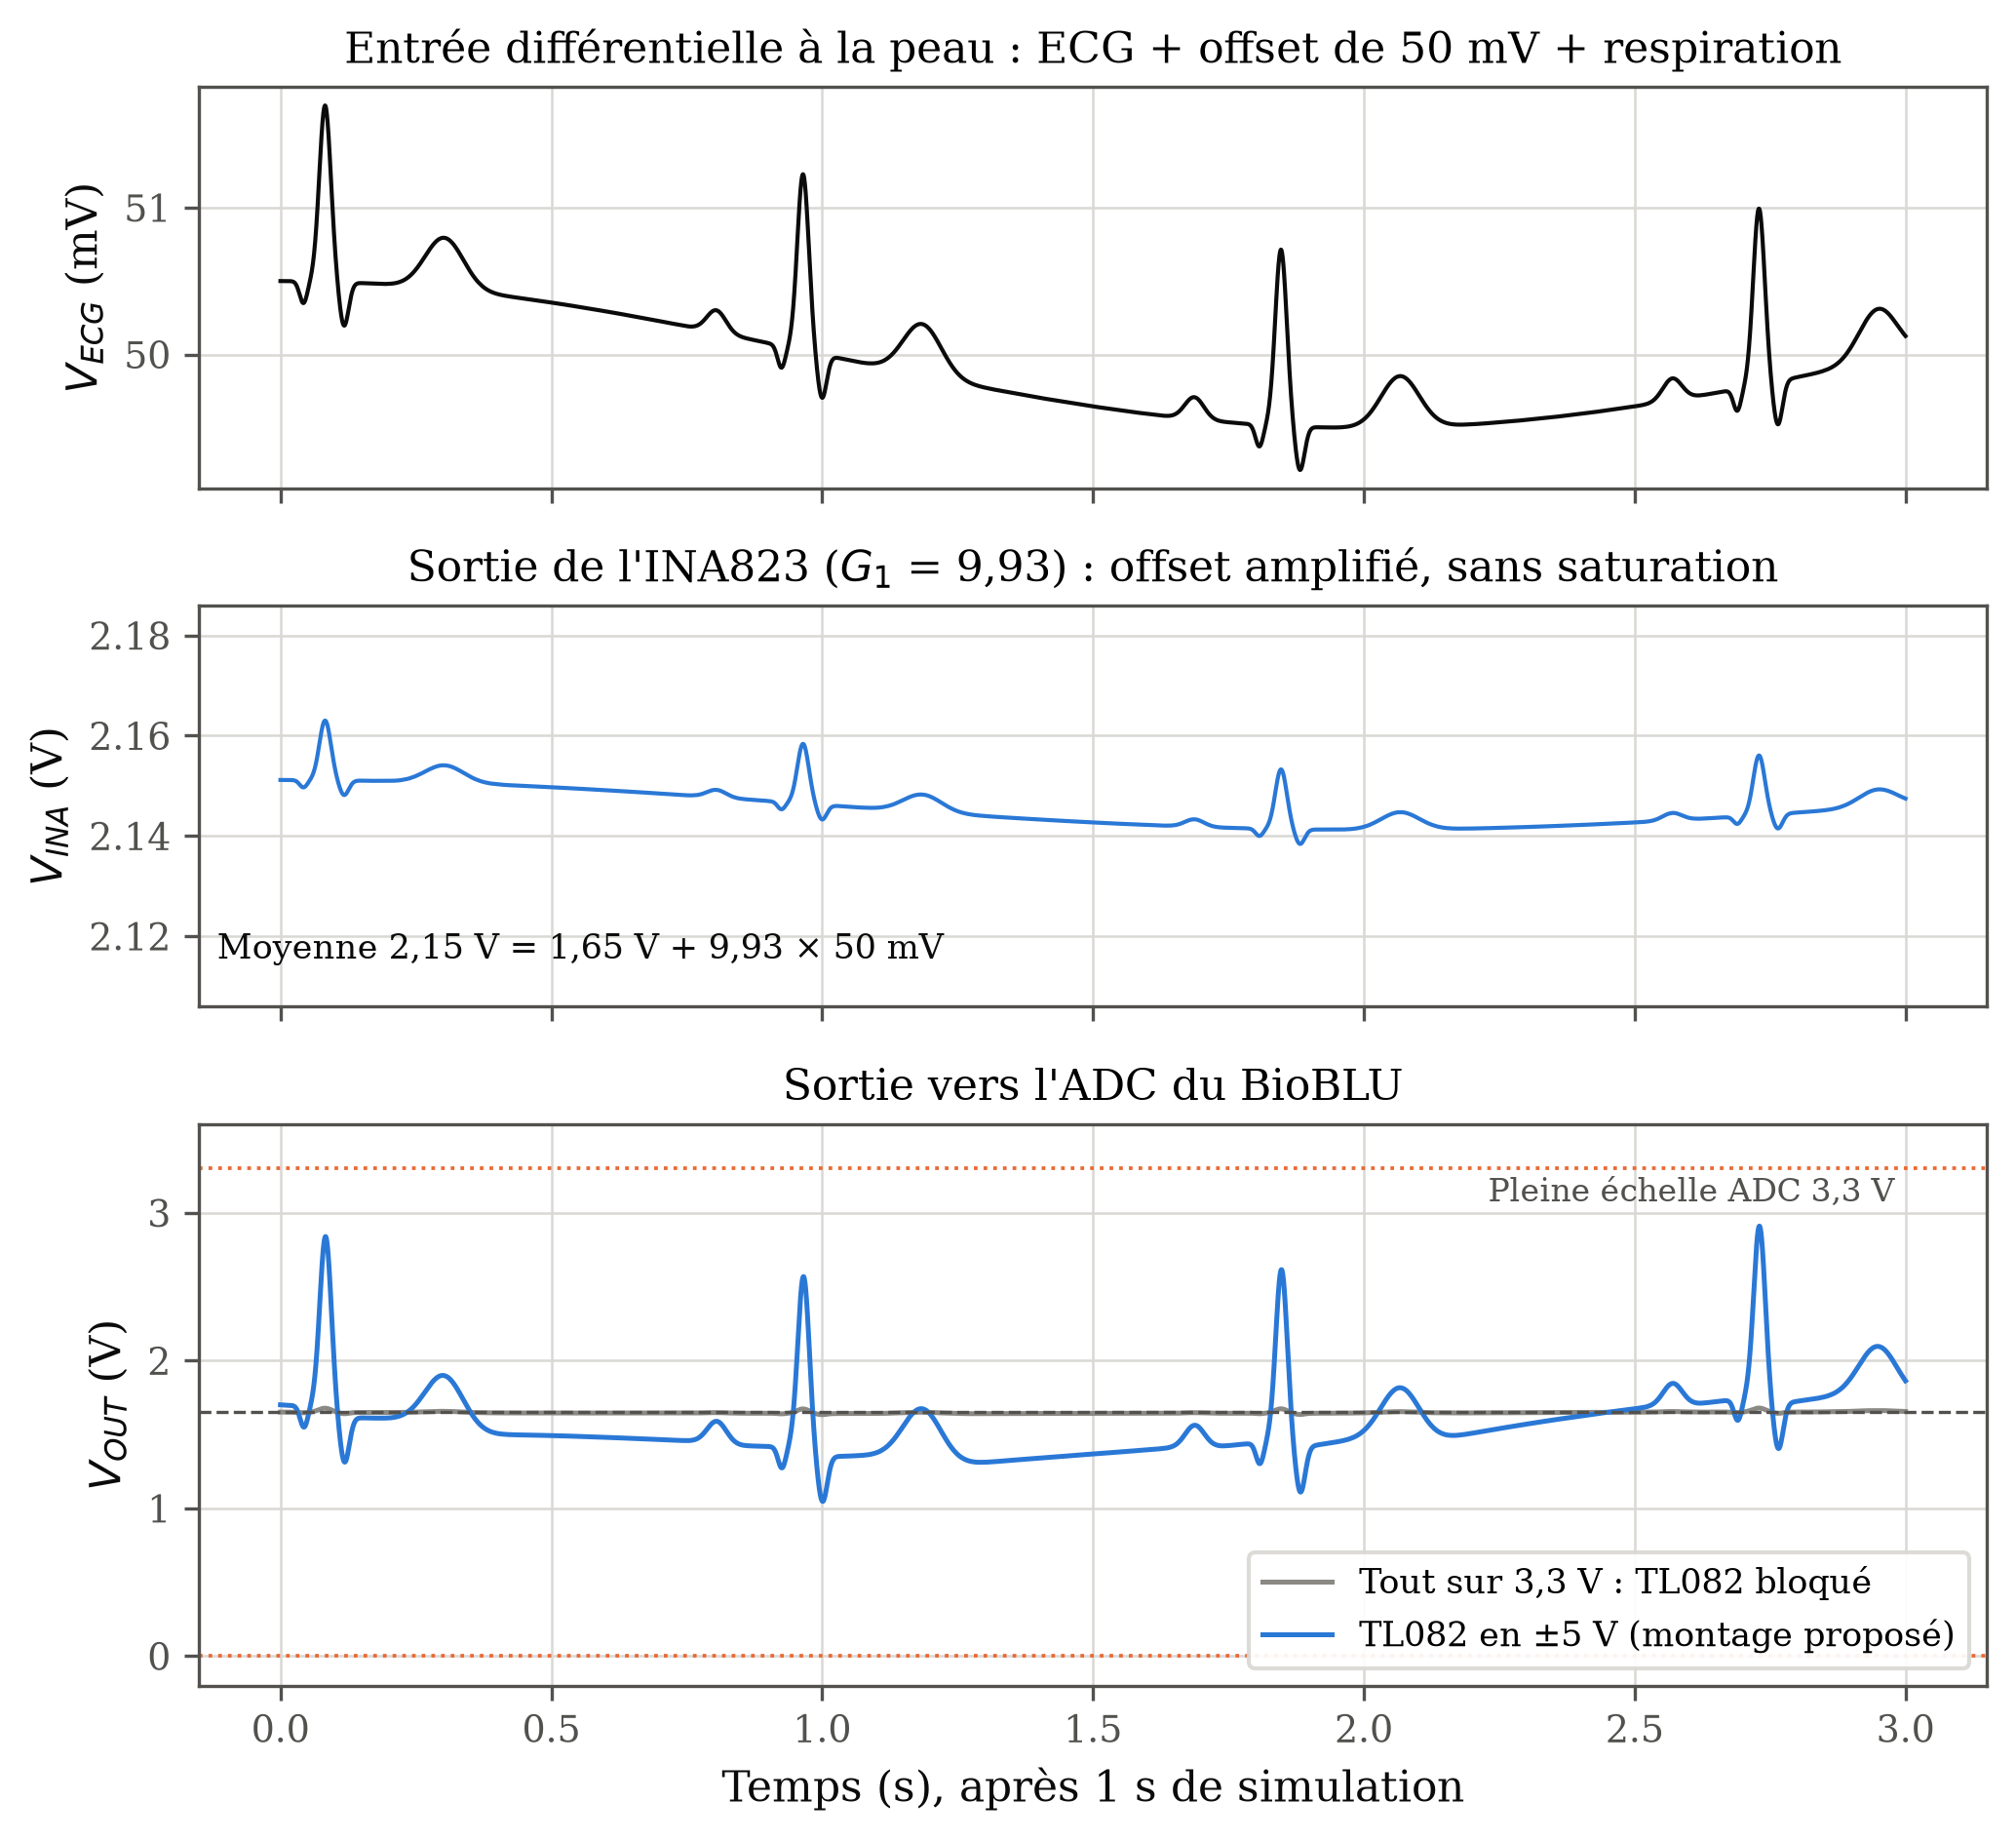
\includegraphics[width=0.9\textwidth]{fig_6_2e_temporel.png}
\caption{Simulation temporelle de la chaîne complète (LTspice, modèles TI). Haut : entrée différentielle à la peau. Milieu : sortie de l'INA823. Bas : sortie vers l'ADC avec les TL082 en $\pm 5\text{ V}$ et lorsque tout est alimenté en $3,3\text{ V}$.}
\label{fig:sim_temporelle}
\end{figure}

En résumé, avec les TL082 alimentés en $\pm 5\text{ V}$, la conception simulée respecte les spécifications du Tableau~\ref{tab:specifications} : gain de $60,0\text{ dB}$, bande passante de $0,48$ à $157\text{ Hz}$, sortie centrée sur $V_{ref}$ dans la plage de l'ADC et $60\text{ Hz}$ résiduel de l'ordre de $0,1\text{ mV}$ en sortie. Le choix de l'alimentation des TL082 reste à confirmer avec les assistants de laboratoire.

\bigskip
{\small\noindent\textbf{Disclaimer} : Nous avons utilisé Claude (Anthropic) pour la mise en page en \LaTeX{}, l'écriture des netlists LTspice et du script de traitement des résultats, l'analyse des simulations et la mise en forme des figures.}

\section*{Références}
\begin{itemize}\sloppy
\item Texas Instruments, \og  Improving common-mode rejection using the right-leg drive amplifier \fg{}, Application Report SBAA188, 2011.
\item Texas Instruments, \og  INA823 Precision, Low-Power, Low-Noise, Instrumentation Amplifier \fg{}, Datasheet SBOSA75B, 2021.
\item Texas Instruments, \og  TL08xx JFET-Input Operational Amplifiers \fg{}, Datasheet SLOS081N, 2023.
\item Texas Instruments, \og  INA823 PSpice Model \fg{} (SBOMBU8B, rév.~B, 2023) et \og  TL082, TL082A, TL082B PSpice Model \fg{} (SLOJ070).
\item Analog Devices, LTspice 26.0.2 pour macOS.
\item M. R. Neuman, \og  Biopotential electrodes \fg{}, \emph{Medical Instrumentation: Application and Design}, 4th ed., J. G. Webster, Ed., John Wiley \& Sons, New York, p. 189--240, 1998.
\item E. Huigen, A. Peper et C. A. Grimbergen, \og  Investigation into the origin of the noise of surface electrodes \fg{}, \emph{Medical and Biological Engineering and Computing}, vol. 40, p. 332--338, 2002.
\item C. Kitchin, L. Counts et M. Gerstenhaber, \og  Reducing RFI rectification errors in in-amp circuits \fg{}, Analog Devices Application Note AN-671, 2003.
\item K. Bouzid et B. Gosselin, \emph{Laboratoire 4 : Bioélectronique -- filtrage et interfaces}, GEL-4072/GEL-7072, Université Laval, automne 2026.
\item B. Gosselin, \emph{Bioamplificateurs et instrumentation de biopotentiels}, Notes de cours GEL-4072/7072, Université Laval, 2024.
\end{itemize}

\end{document}

